\chapterimage{chap3.jpg}
\chapter{栈和队列}
\section{栈}
\begin{definition}[栈]
    \begin{enumerate}
        \item 只允许在一端进行插入和删除操作的线性表
        \item 栈有栈顶、栈底两个重要元素,栈顶元素是最后一个插入的元素,栈底元素是最先插入的元素
        \item 栈的插入操作叫做进栈,栈的删除操作叫做出栈
        \item 栈的特点是后进先出,简称 $\mathbf{LIFO}, \mathbf{Last\ In\ First\ Out}$
        \item $n$ 个不同元素进栈, 出栈元素不同的排列个数: $\mathbf{Catalan}(n) = \dfrac{1}{n+1}\binom{n}{2n}$
    \end{enumerate}
\end{definition}

\begin{definition}[栈基本操作]
    \begin{enumerate}
        \item $\mathbf{InitStack(\& S)}$  初始化栈 $S$
        \item $\mathbf{DestroyStack(\& S)}$  销毁栈 $S$
        \item $\mathbf{GetTop(S,\&e)}$ 获取栈顶元素,将栈 $S$ 的栈顶元素赋值给 $e$
        \item $\mathbf{Push(\&S,e)}$ 压栈
        \item $\mathbf{Pop(\&S,\&e)}$ 出栈
        \item $\mathbf{Length(S)}$ 求栈中元素个数
        \item $\mathbf{Empty(S)}$ 判空
        \item $\mathbf{PrintStack(S)}$ 输出操作,输出栈 $S$ 的所有元素 
    \end{enumerate}
\end{definition}
\subsection{栈定义和函数声明}

\subsubsection{顺序栈、链栈、共享栈定义}

\begin{figure}[H]
    \centering
    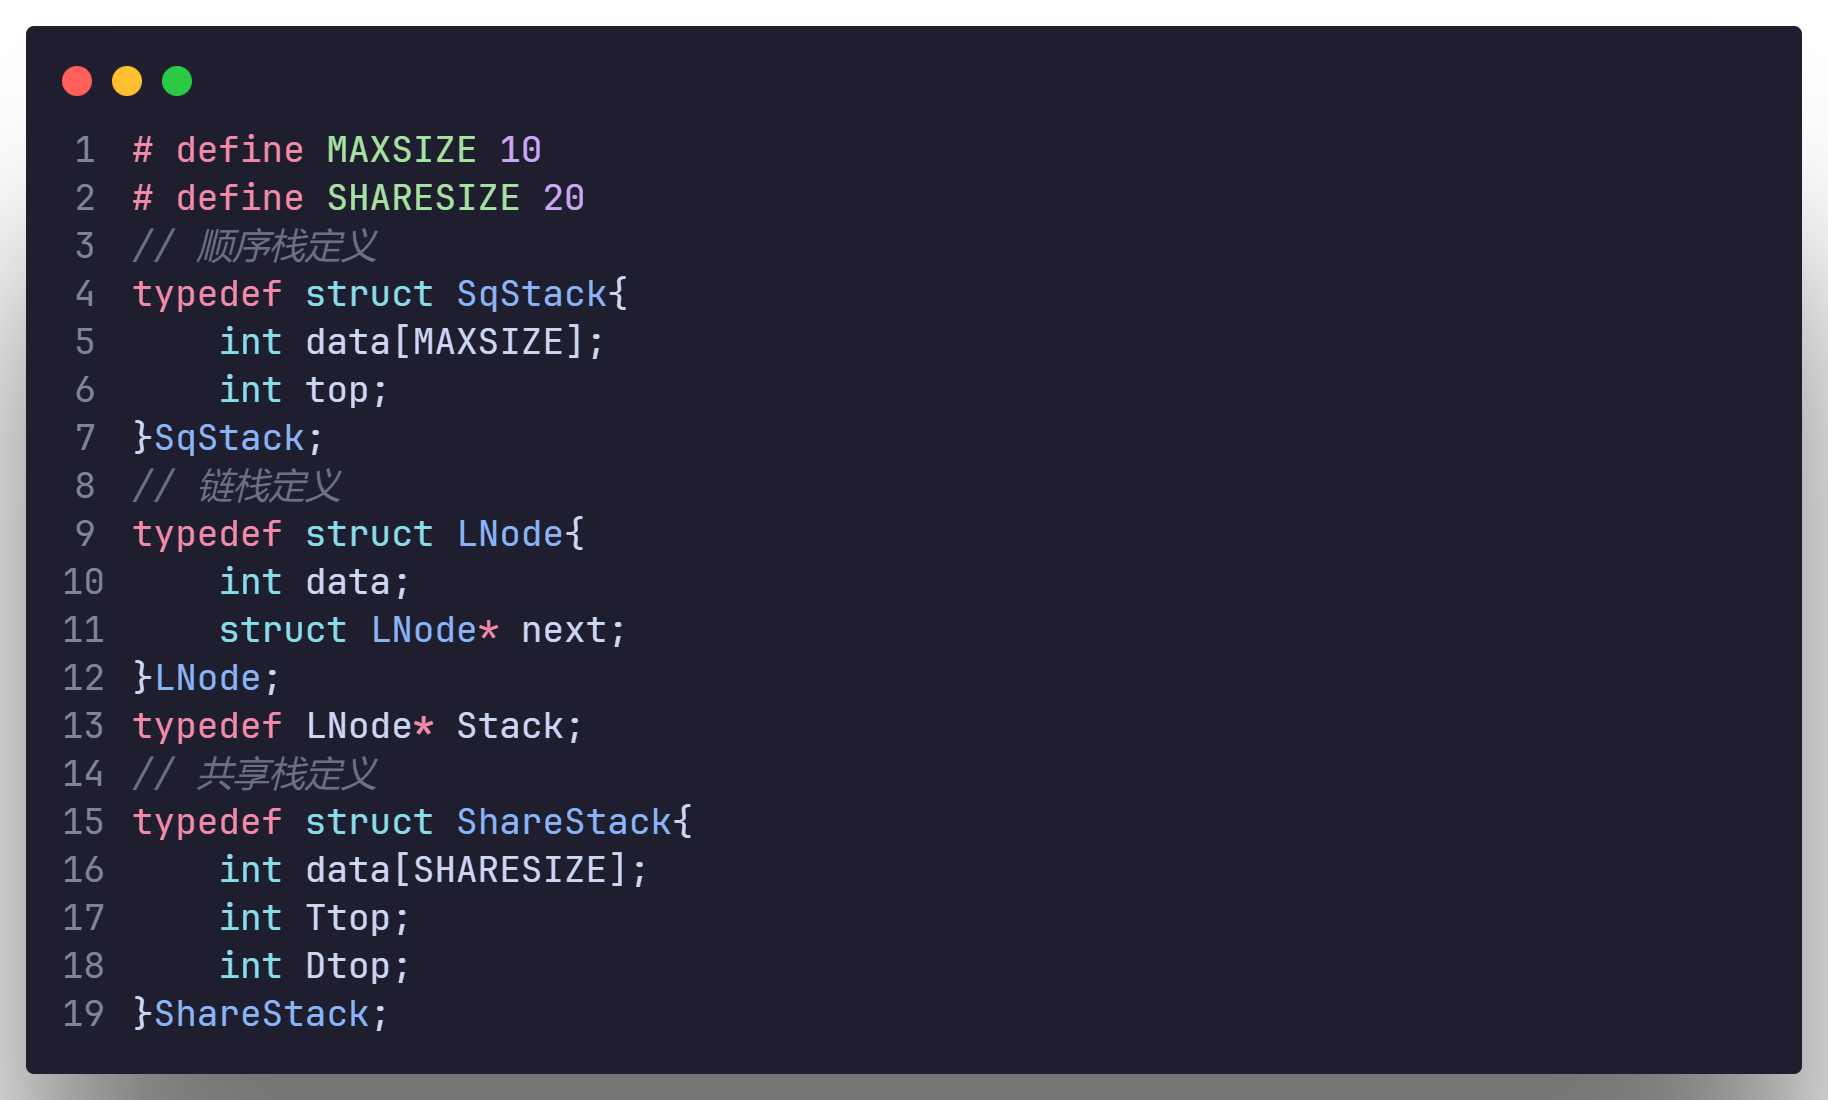
\includegraphics[scale=0.2]{"figure/Note/Stack/SDefine.png"}
\end{figure}

\subsubsection{函数声明}

\begin{figure}[H]
    \centering
    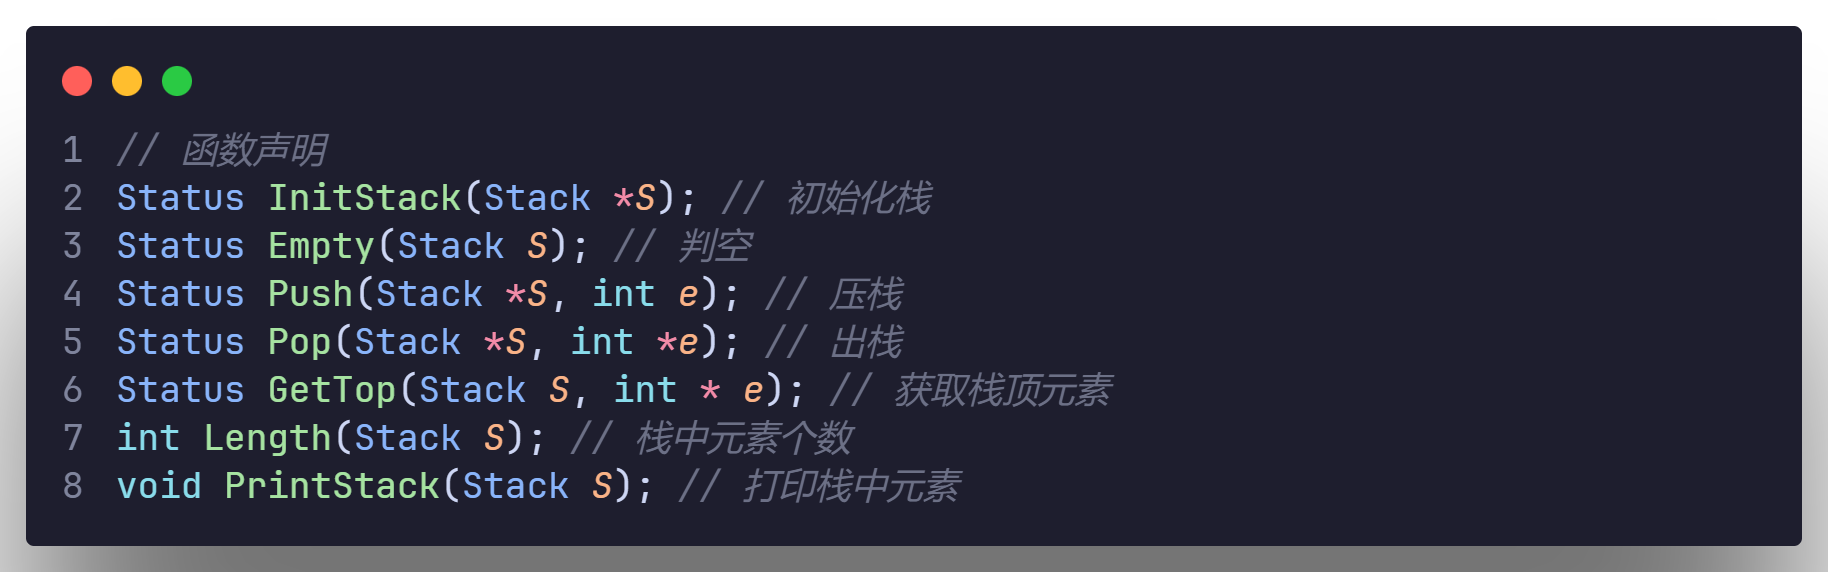
\includegraphics[scale=0.2]{"figure/Note/Stack/SFunction.png"}
\end{figure}

\subsection{顺序栈}
\begin{definition}[顺序栈]
    顺序栈是用顺序表实现的栈,使用 $\mathbf{top}$ 指针指定栈顶元素在顺序表中的位置,栈的容量大小固定, 需要判空和判满.
\end{definition}

\subsubsection{顺序栈初始化}

\begin{figure}[H]
    \centering
    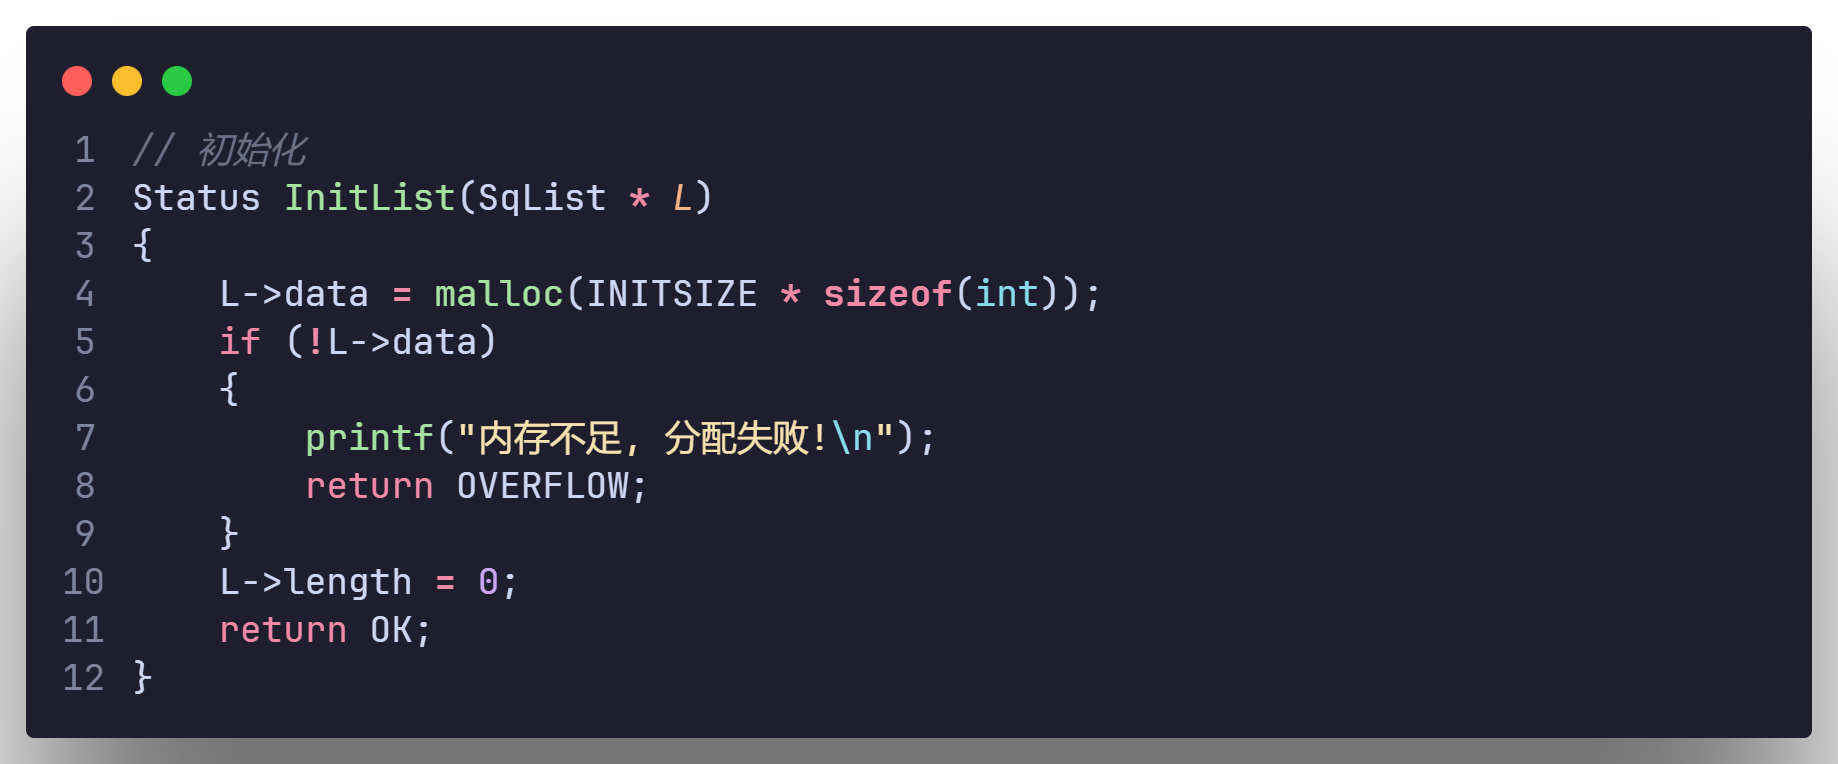
\includegraphics[scale=0.2]{"figure/Note/Stack/SqInit.png"}
\end{figure}

\subsubsection{顺序栈出入栈}

\begin{figure}[H]
    \centering
    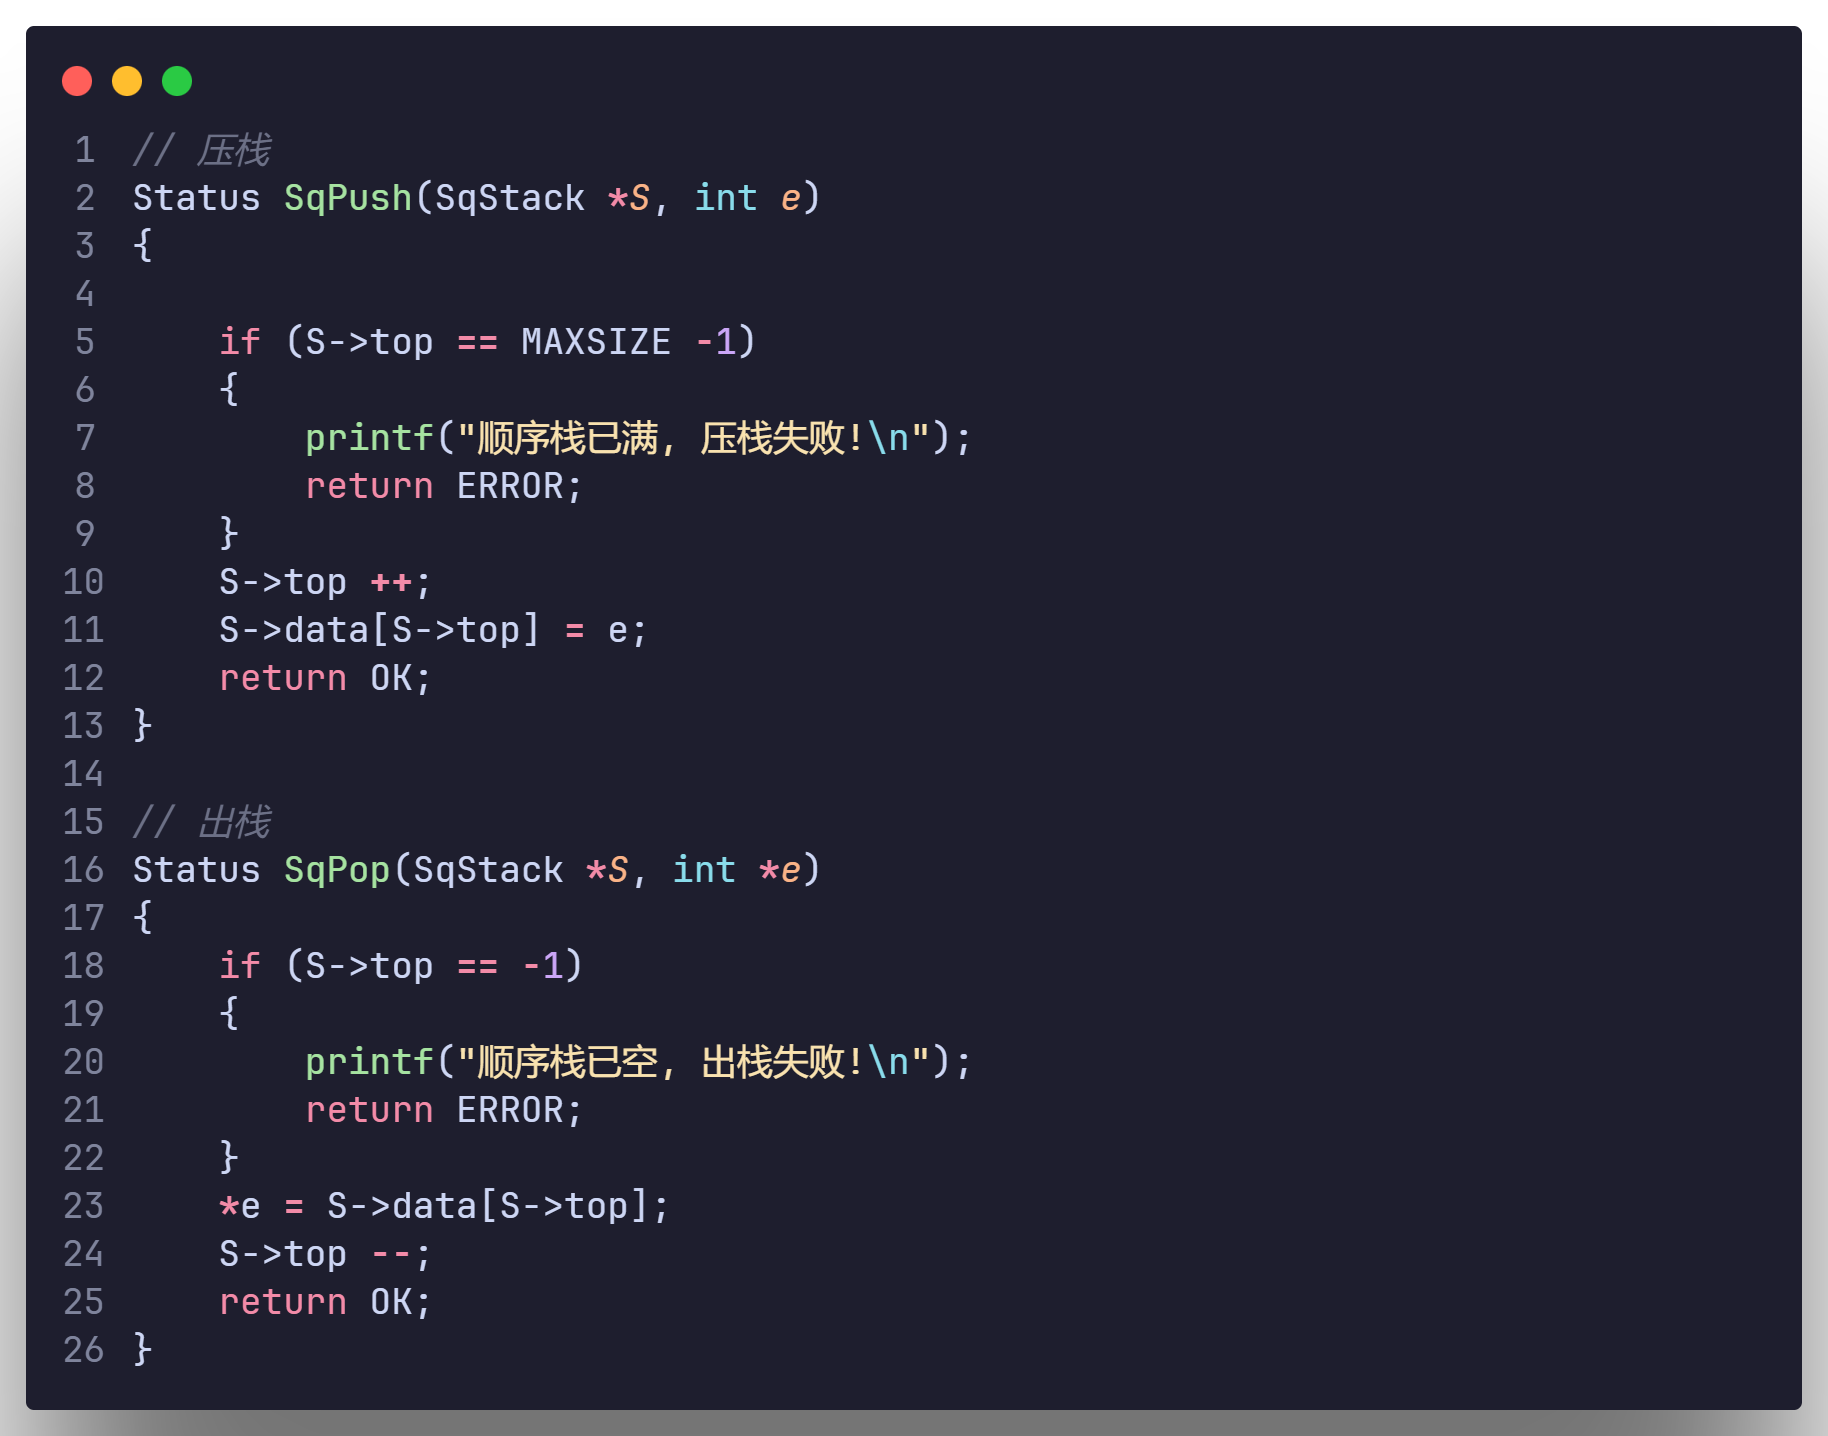
\includegraphics[scale=0.2]{"figure/Note/Stack/SqP.png"}
\end{figure}

\subsubsection{顺序栈辅助函数}

(1). 判断栈是否为空

\begin{figure}[H]
    \centering
    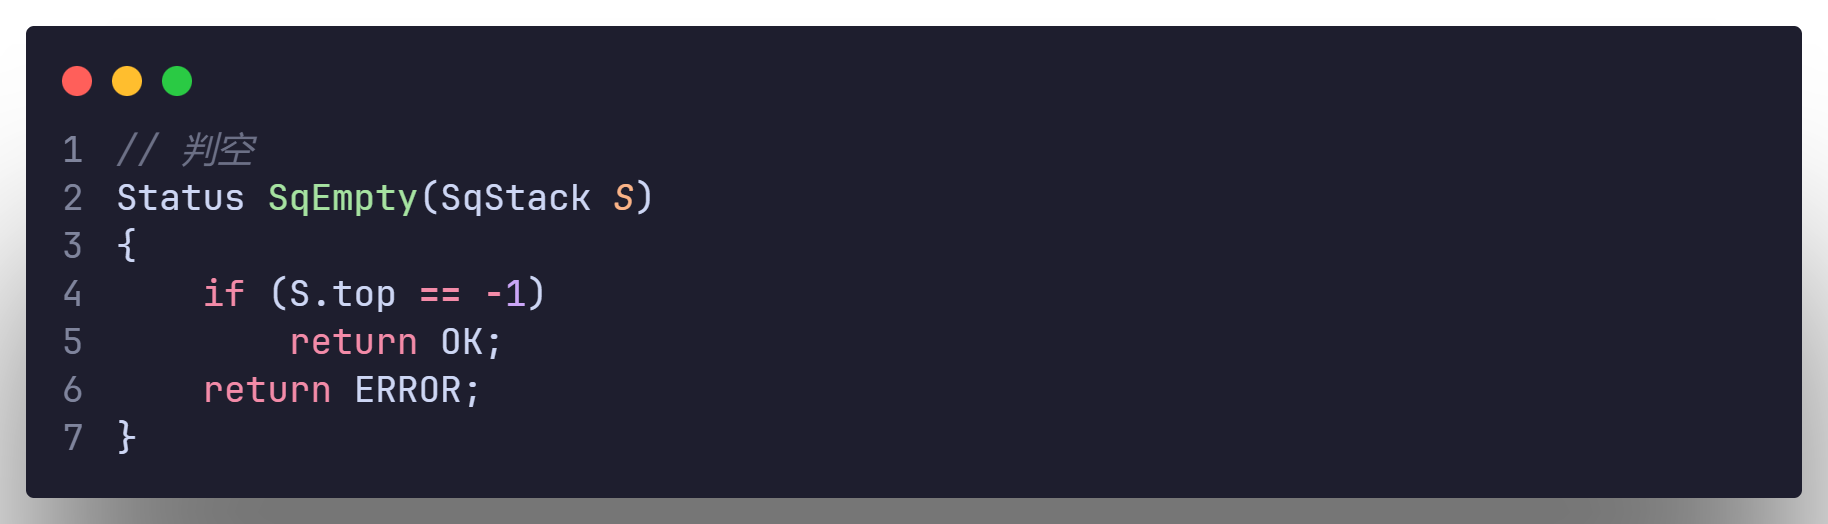
\includegraphics[scale=0.2]{"figure/Note/Stack/SqEmpty.png"}
\end{figure}

(2). 获取栈顶元素

\begin{figure}[H]
    \centering
    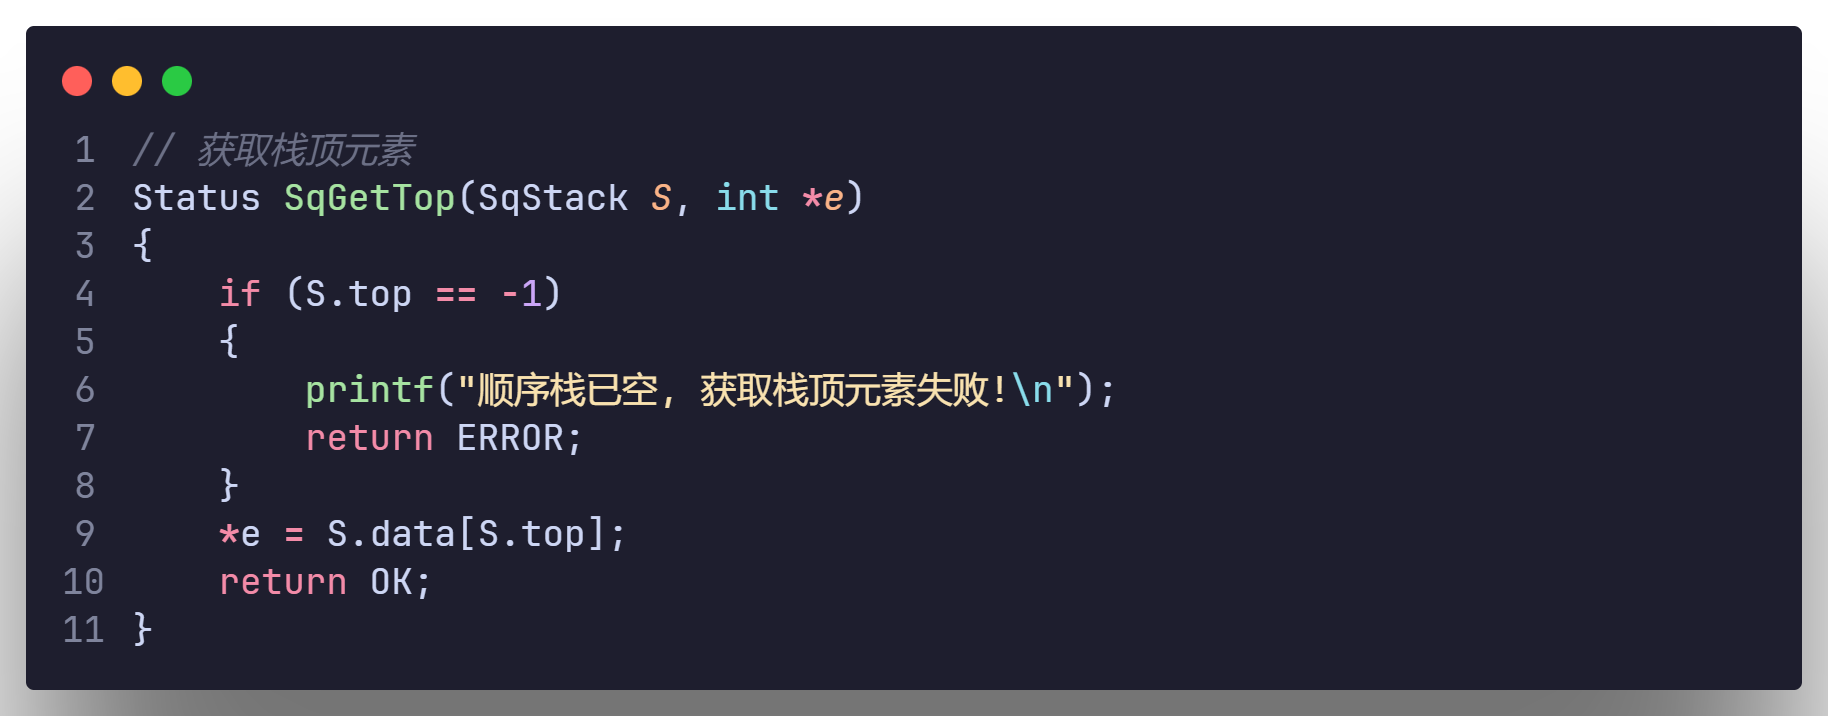
\includegraphics[scale=0.2]{"figure/Note/Stack/SqG.png"}
\end{figure}

(3). 获取栈中元素个数

\begin{figure}[H]
    \centering
    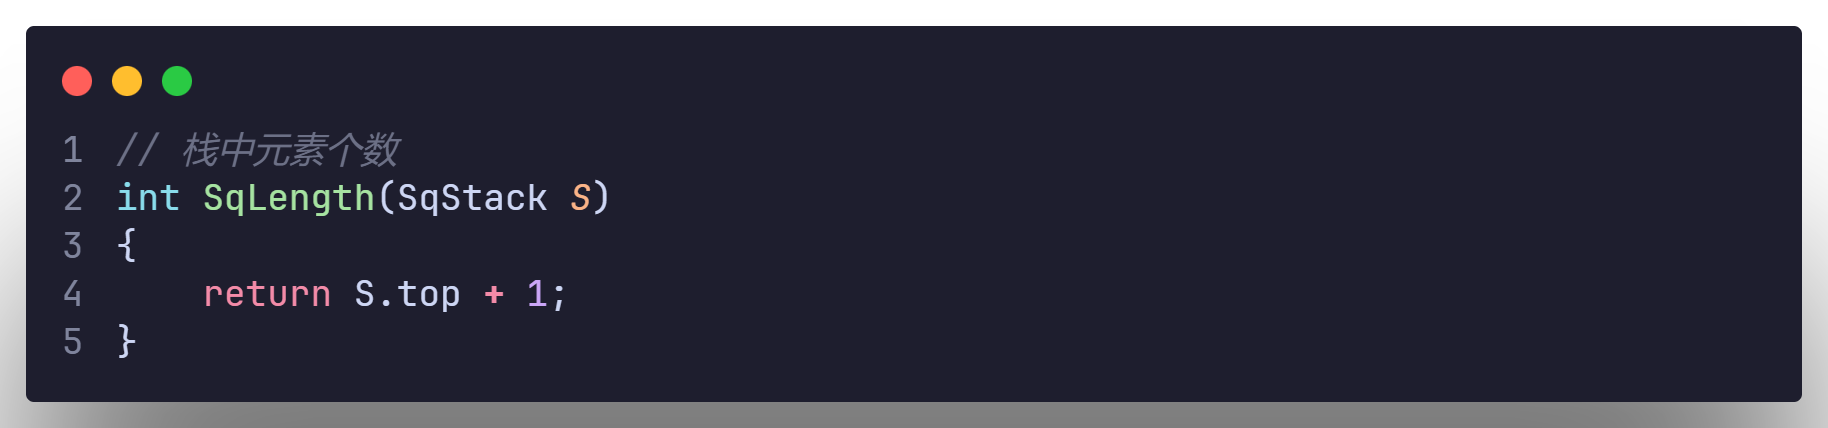
\includegraphics[scale=0.2]{"figure/Note/Stack/SqN.png"}
\end{figure}

(4). 打印栈中元素

\begin{figure}[H]
    \centering
    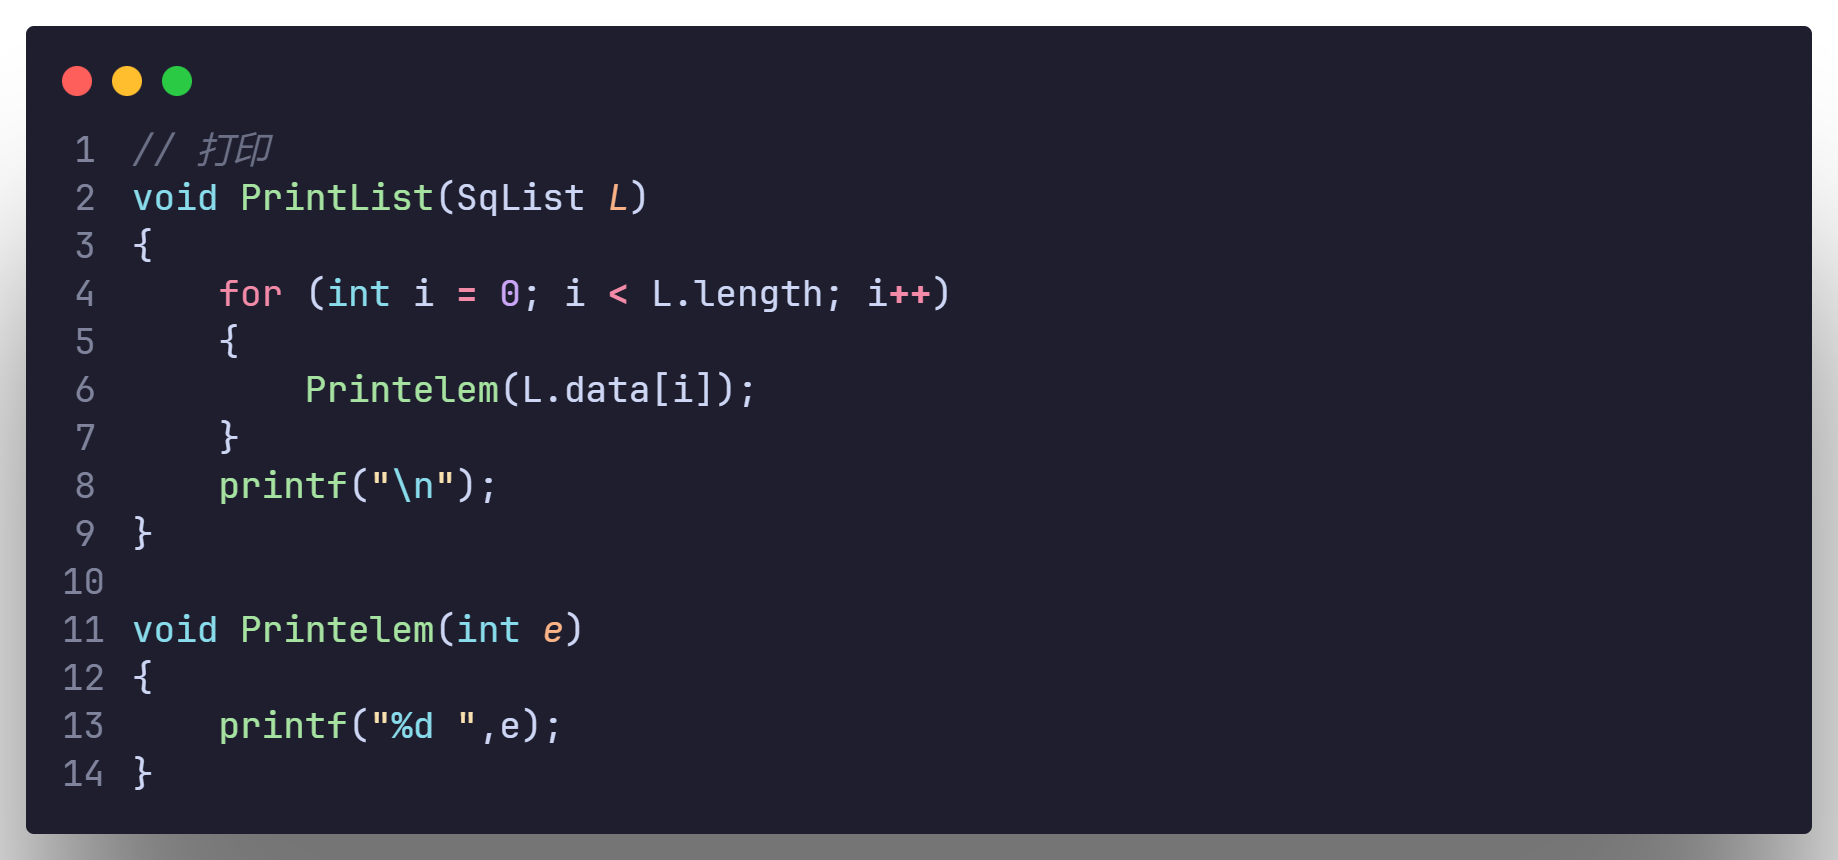
\includegraphics[scale=0.2]{"figure/Note/Stack/SqPrint.png"}
\end{figure}

\subsection{链栈}
\begin{definition}[链栈]
    链栈是使用链表实现的栈,不需要判满,只需要判空,出栈和入栈操作都在链表的头部进行,只需要表头指针,一般使用不带头节点的单链表实现.
\end{definition}

\subsubsection{链栈初始化}

\begin{figure}[H]
    \centering
    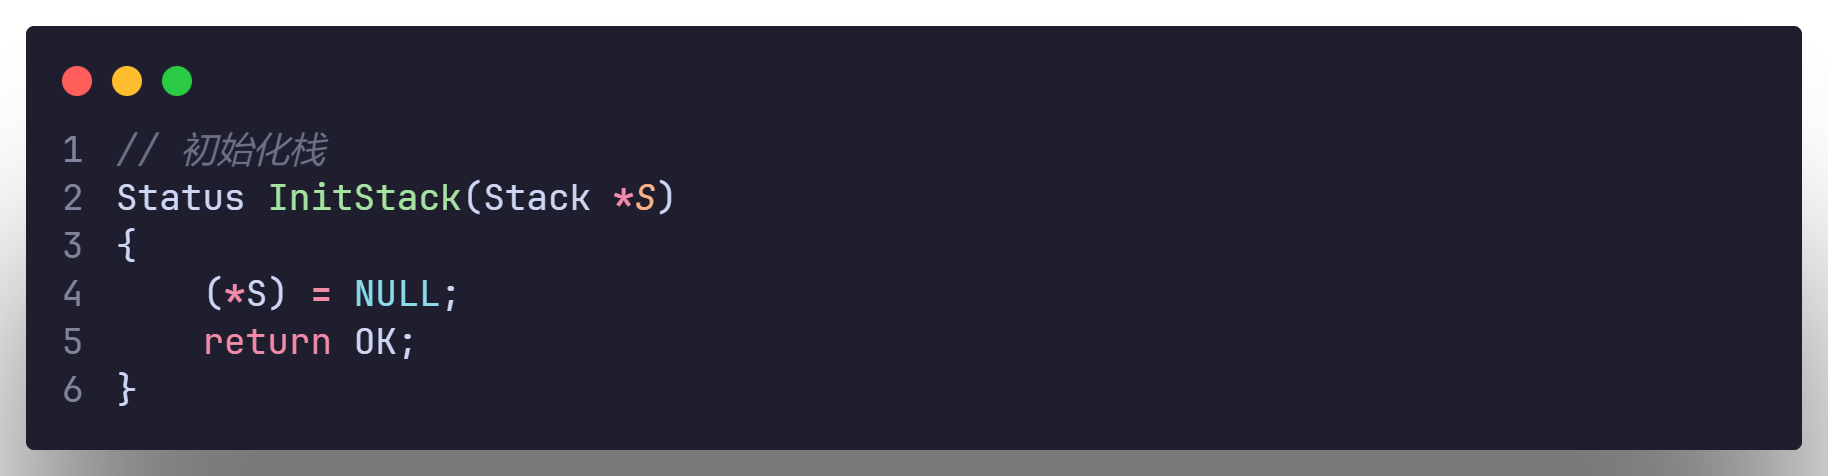
\includegraphics[scale=0.2]{"figure/Note/Stack/SlInit.png"}
\end{figure}

\subsubsection{链栈出入栈}

\begin{figure}[H]
    \centering
    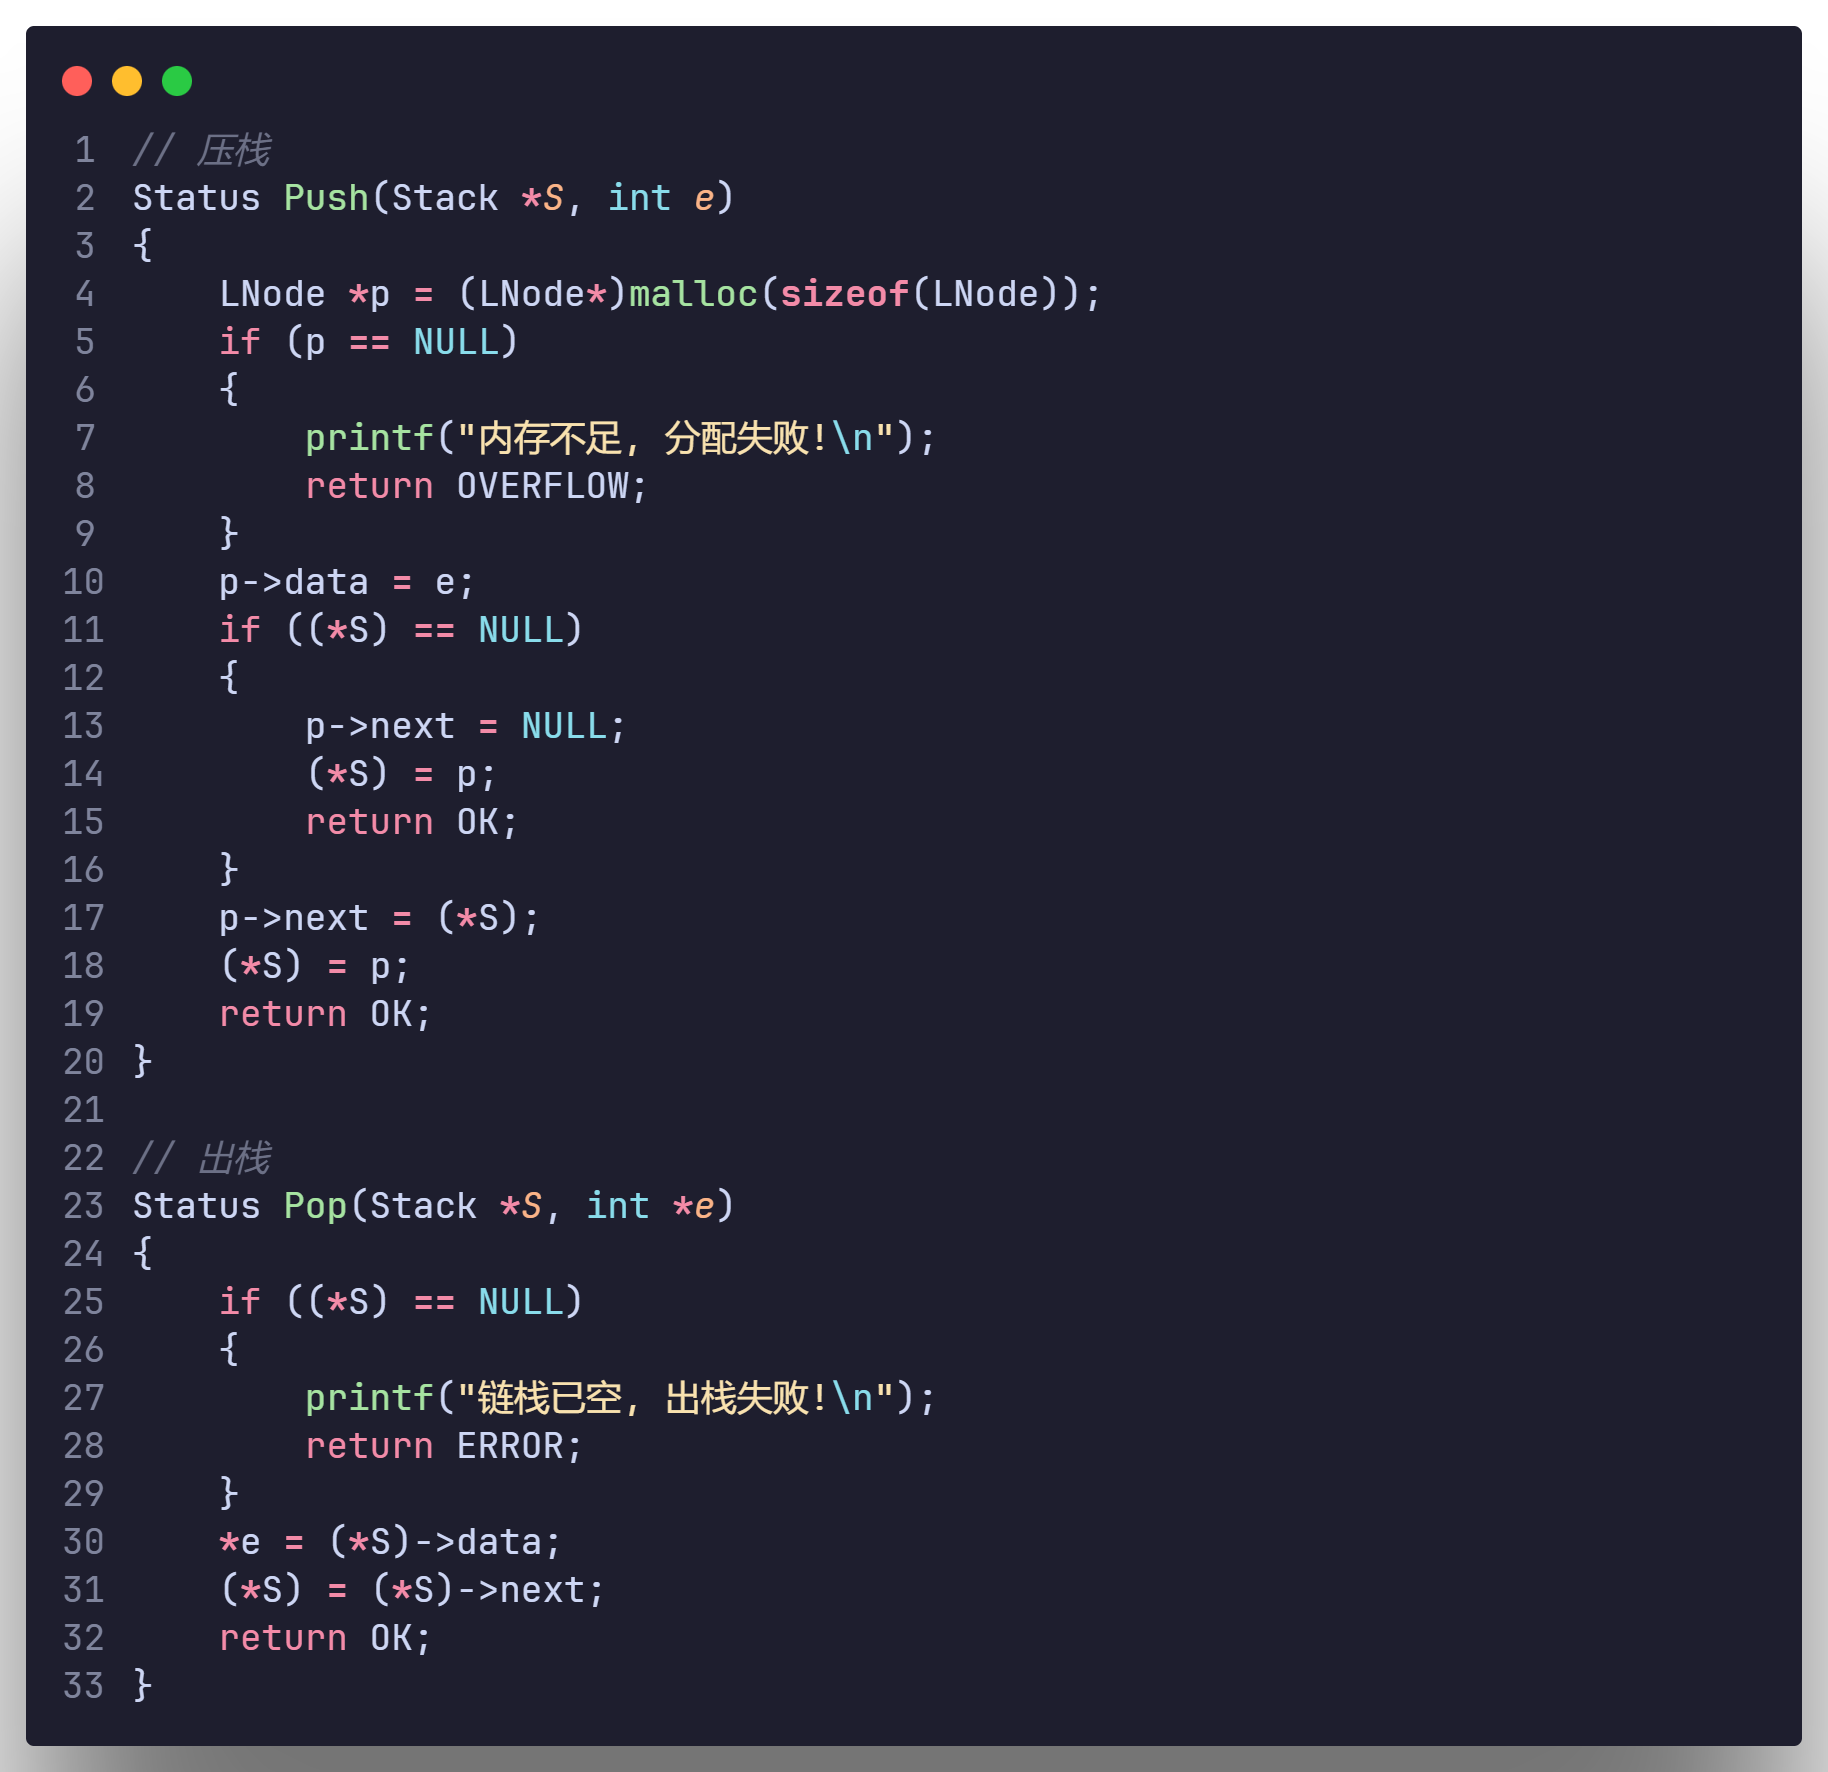
\includegraphics[scale=0.2]{"figure/Note/Stack/SlP.png"}
\end{figure}

\subsubsection{链栈辅助函数}

(1). 判断栈是否为空

\begin{figure}[H]
    \centering
    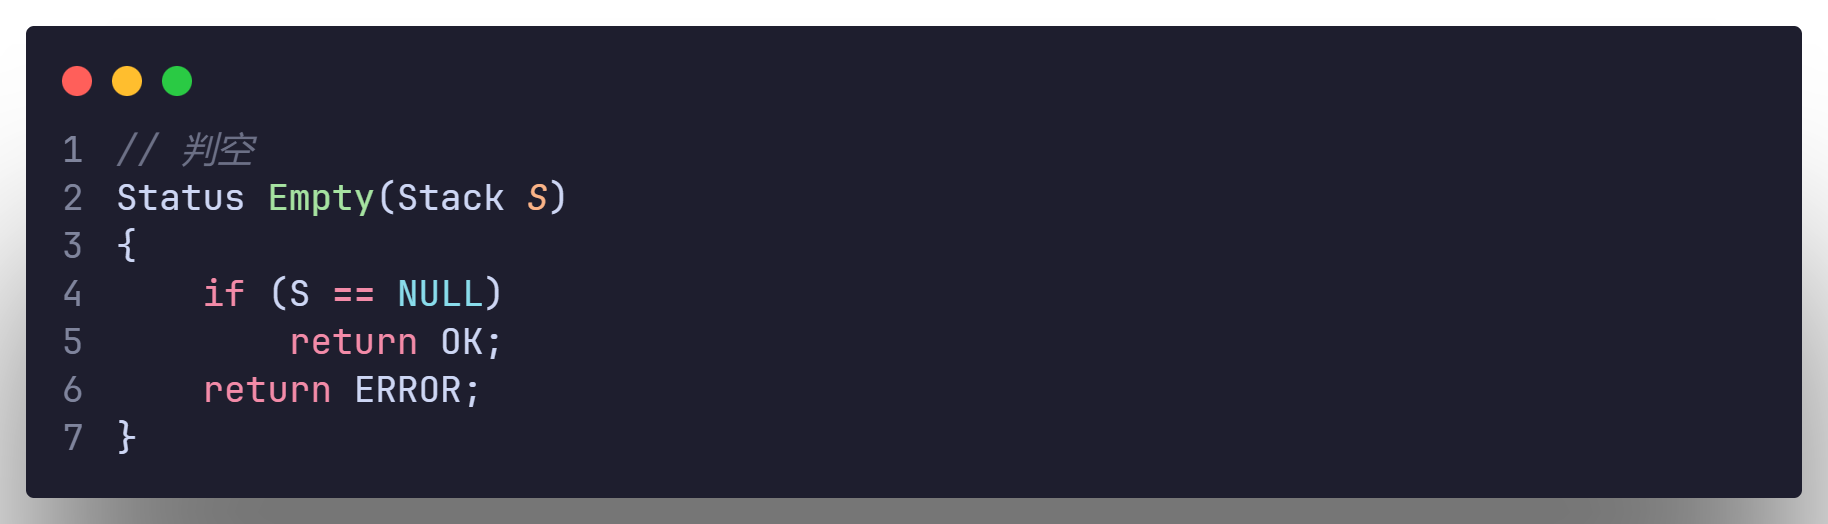
\includegraphics[scale=0.2]{"figure/Note/Stack/SlEmpty.png"}
\end{figure}

(2). 获取栈顶元素

\begin{figure}[H]
    \centering
    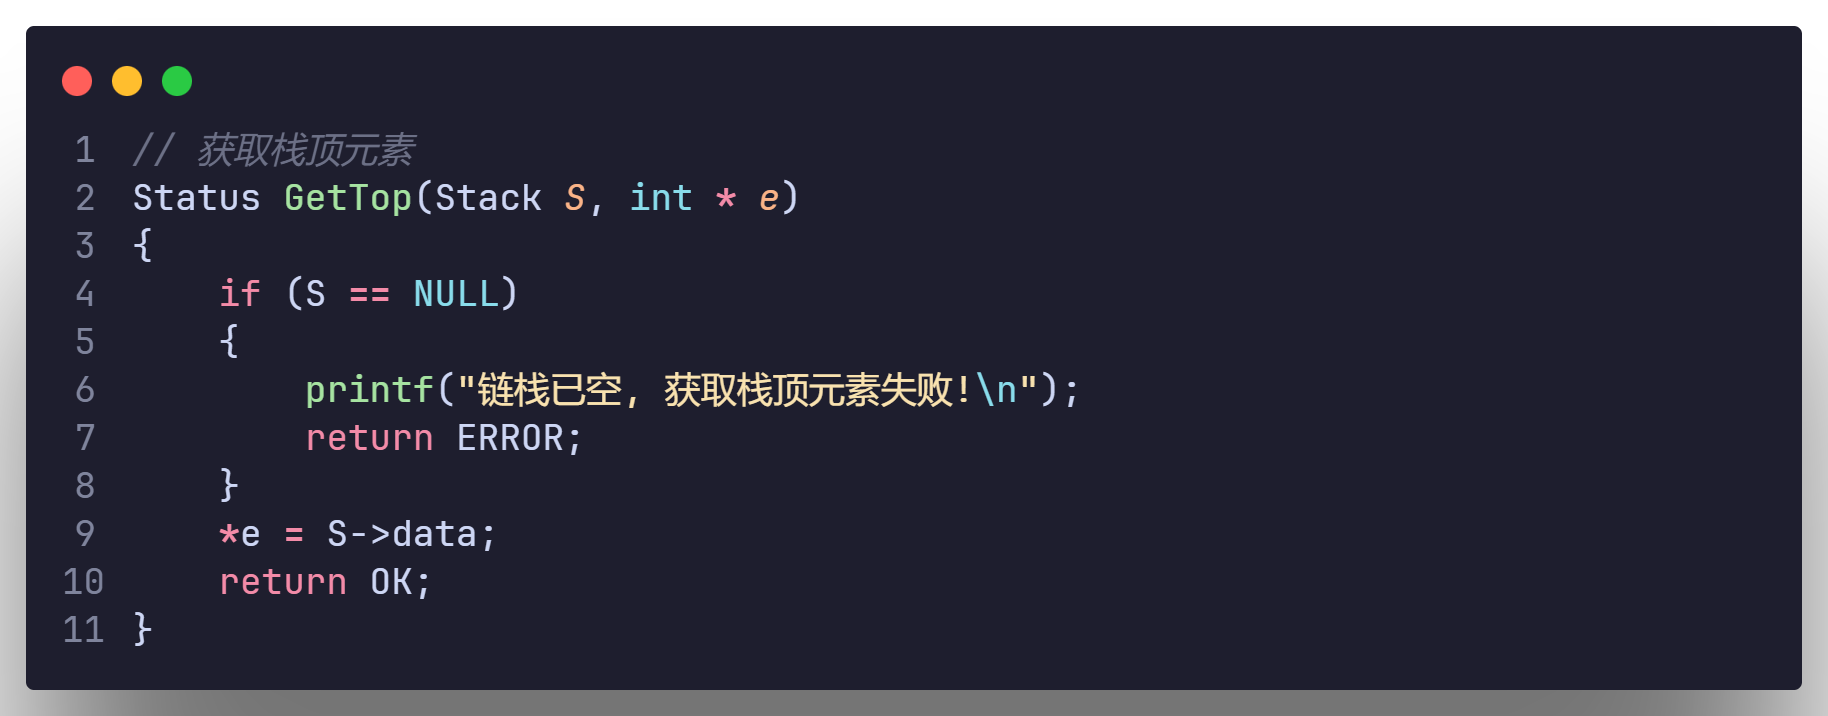
\includegraphics[scale=0.2]{"figure/Note/Stack/SlG.png"}
\end{figure}

(3). 获取栈中元素个数

\begin{figure}[H]
    \centering
    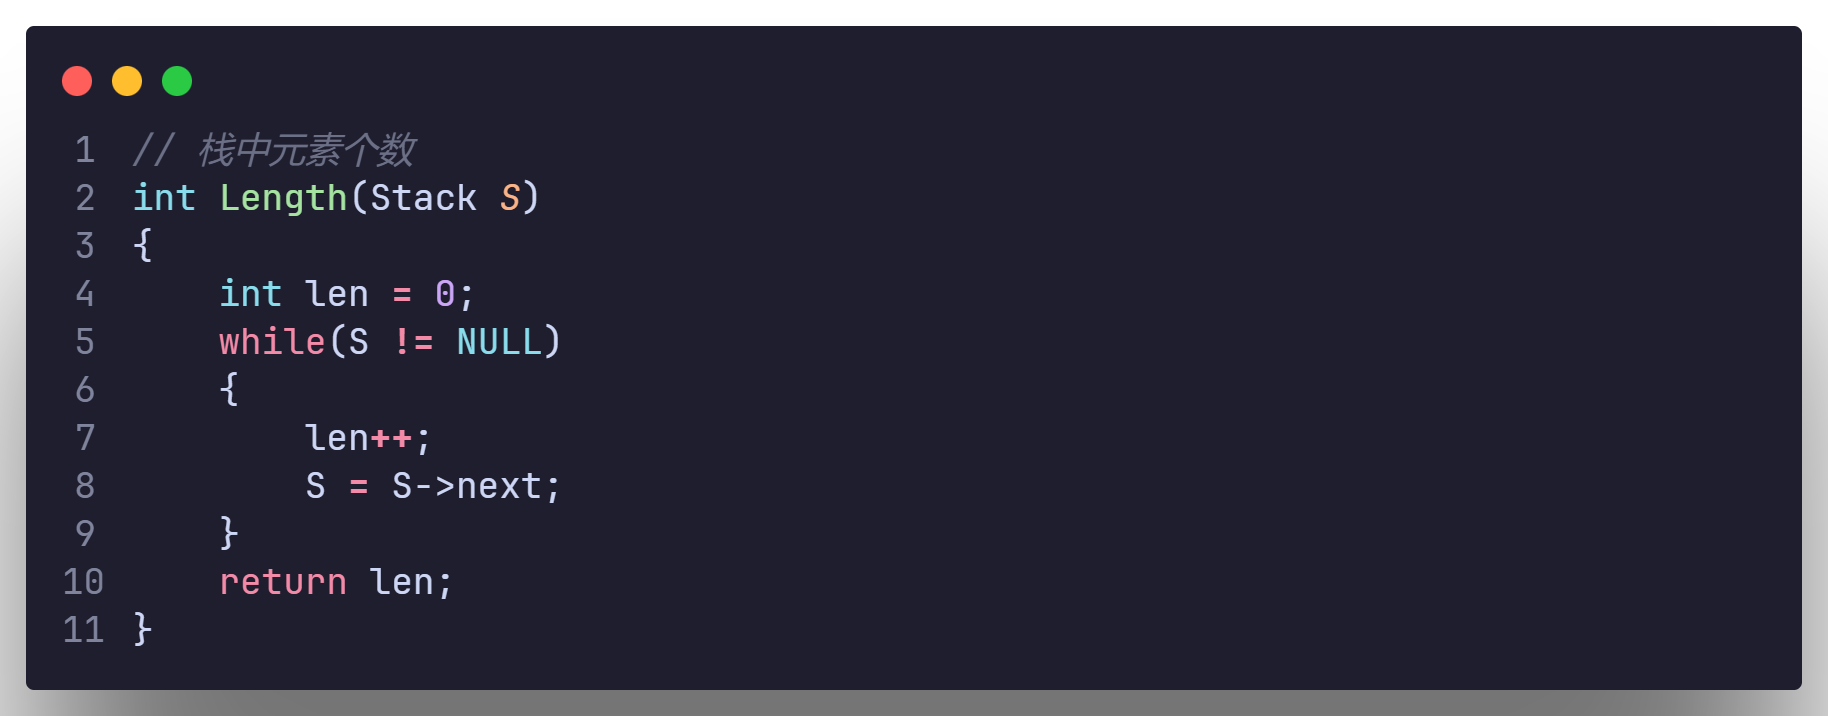
\includegraphics[scale=0.2]{"figure/Note/Stack/SlN.png"}
\end{figure}

(4). 打印栈中元素

\begin{figure}[H]
    \centering
    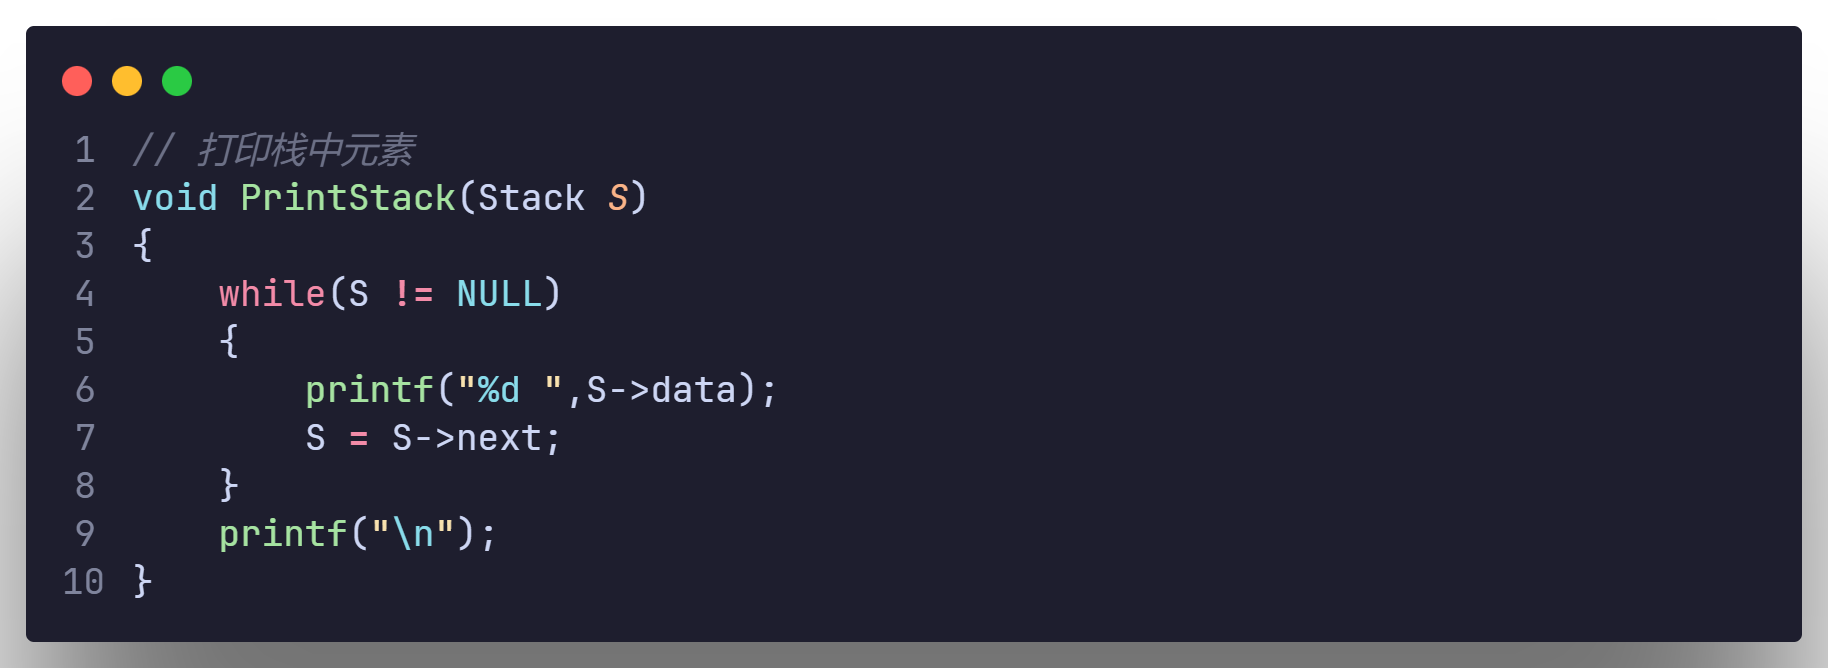
\includegraphics[scale=0.2]{"figure/Note/Stack/SlPrint.png"}
\end{figure}


\subsection{共享栈}
\begin{definition}[共享栈]
    共享栈是两个栈共享一个顺序表,两个栈的栈底分别在顺序表的两端,两个栈的栈顶指针分别向中间移动,当两个栈的栈顶指针相遇时,表示栈满; 共享栈主要是为了充分利用空间,提高空间利用率.
\end{definition}

\subsubsection{共享栈初始化}

\begin{figure}[H]
    \centering
    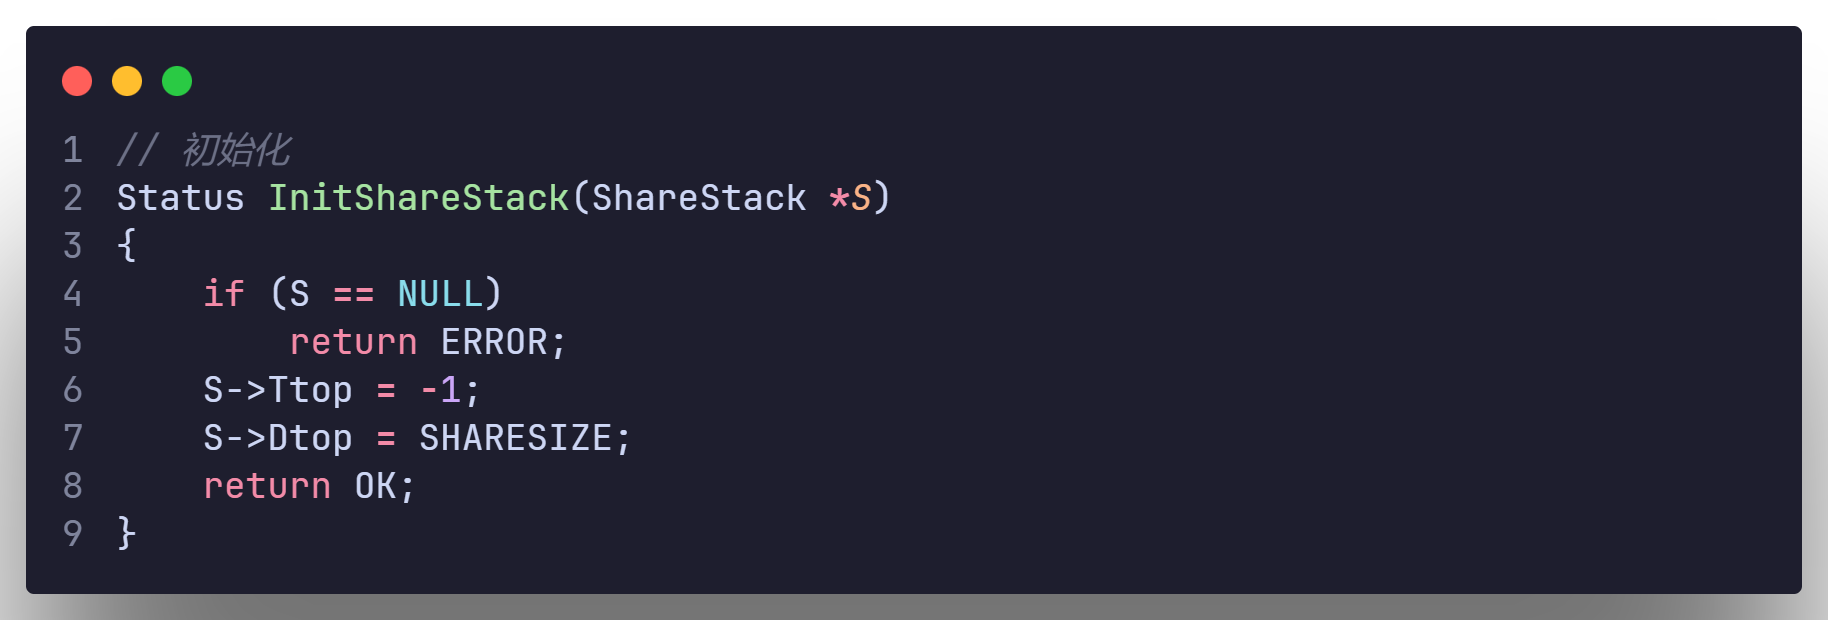
\includegraphics[scale=0.2]{"figure/Note/Stack/SSInit.png"}
\end{figure}

\subsubsection{共享栈出入栈}

(1). 入栈

\begin{figure}[H]
    \centering
    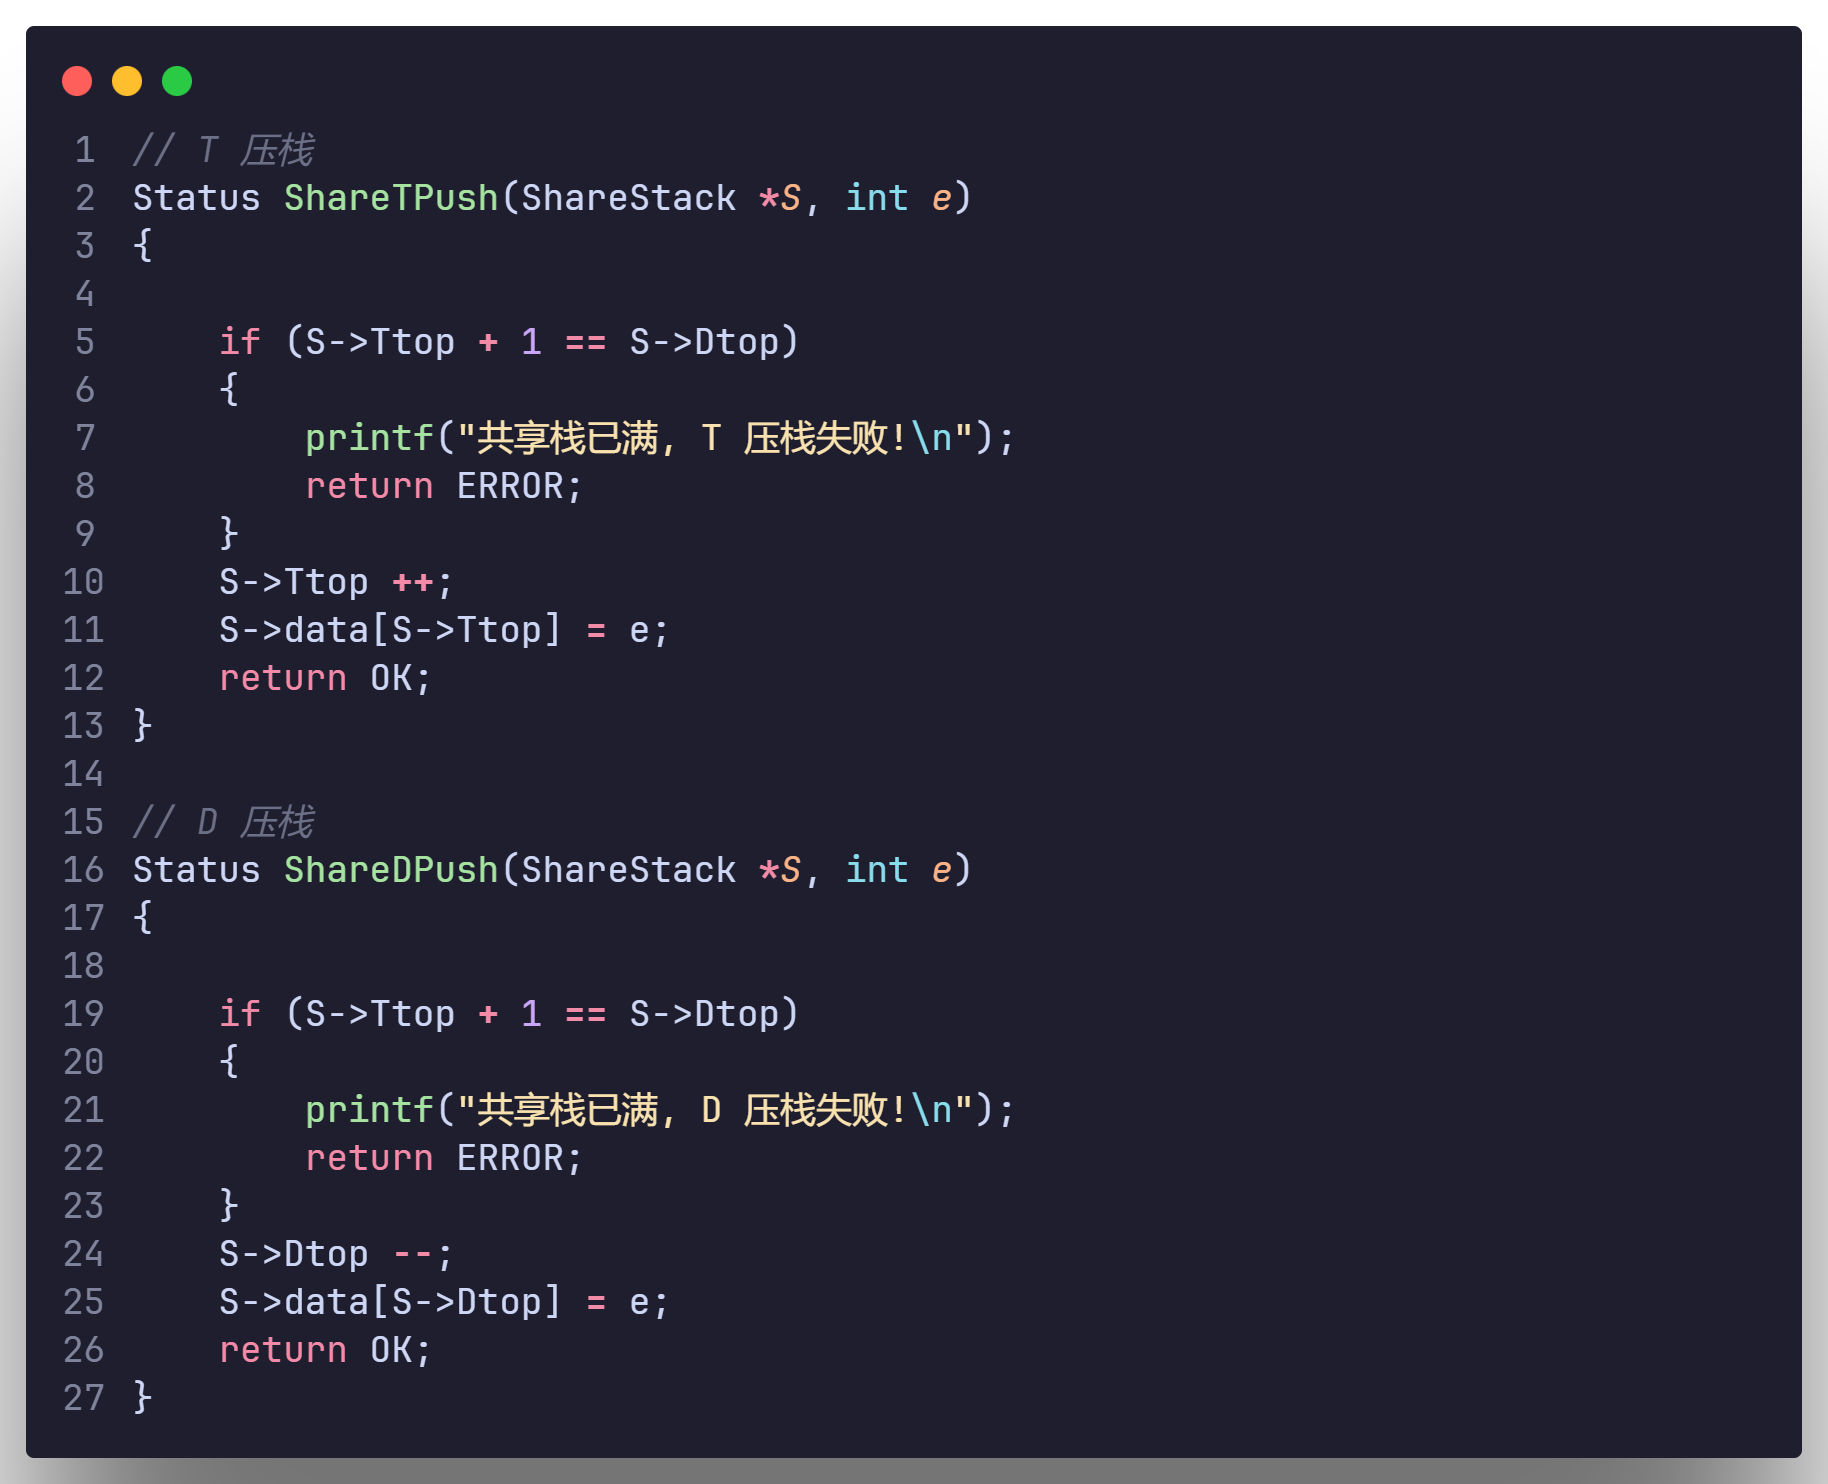
\includegraphics[scale=0.2]{"figure/Note/Stack/SSPush.png"}
\end{figure}

(2). 出栈

\begin{figure}[H]
    \centering
    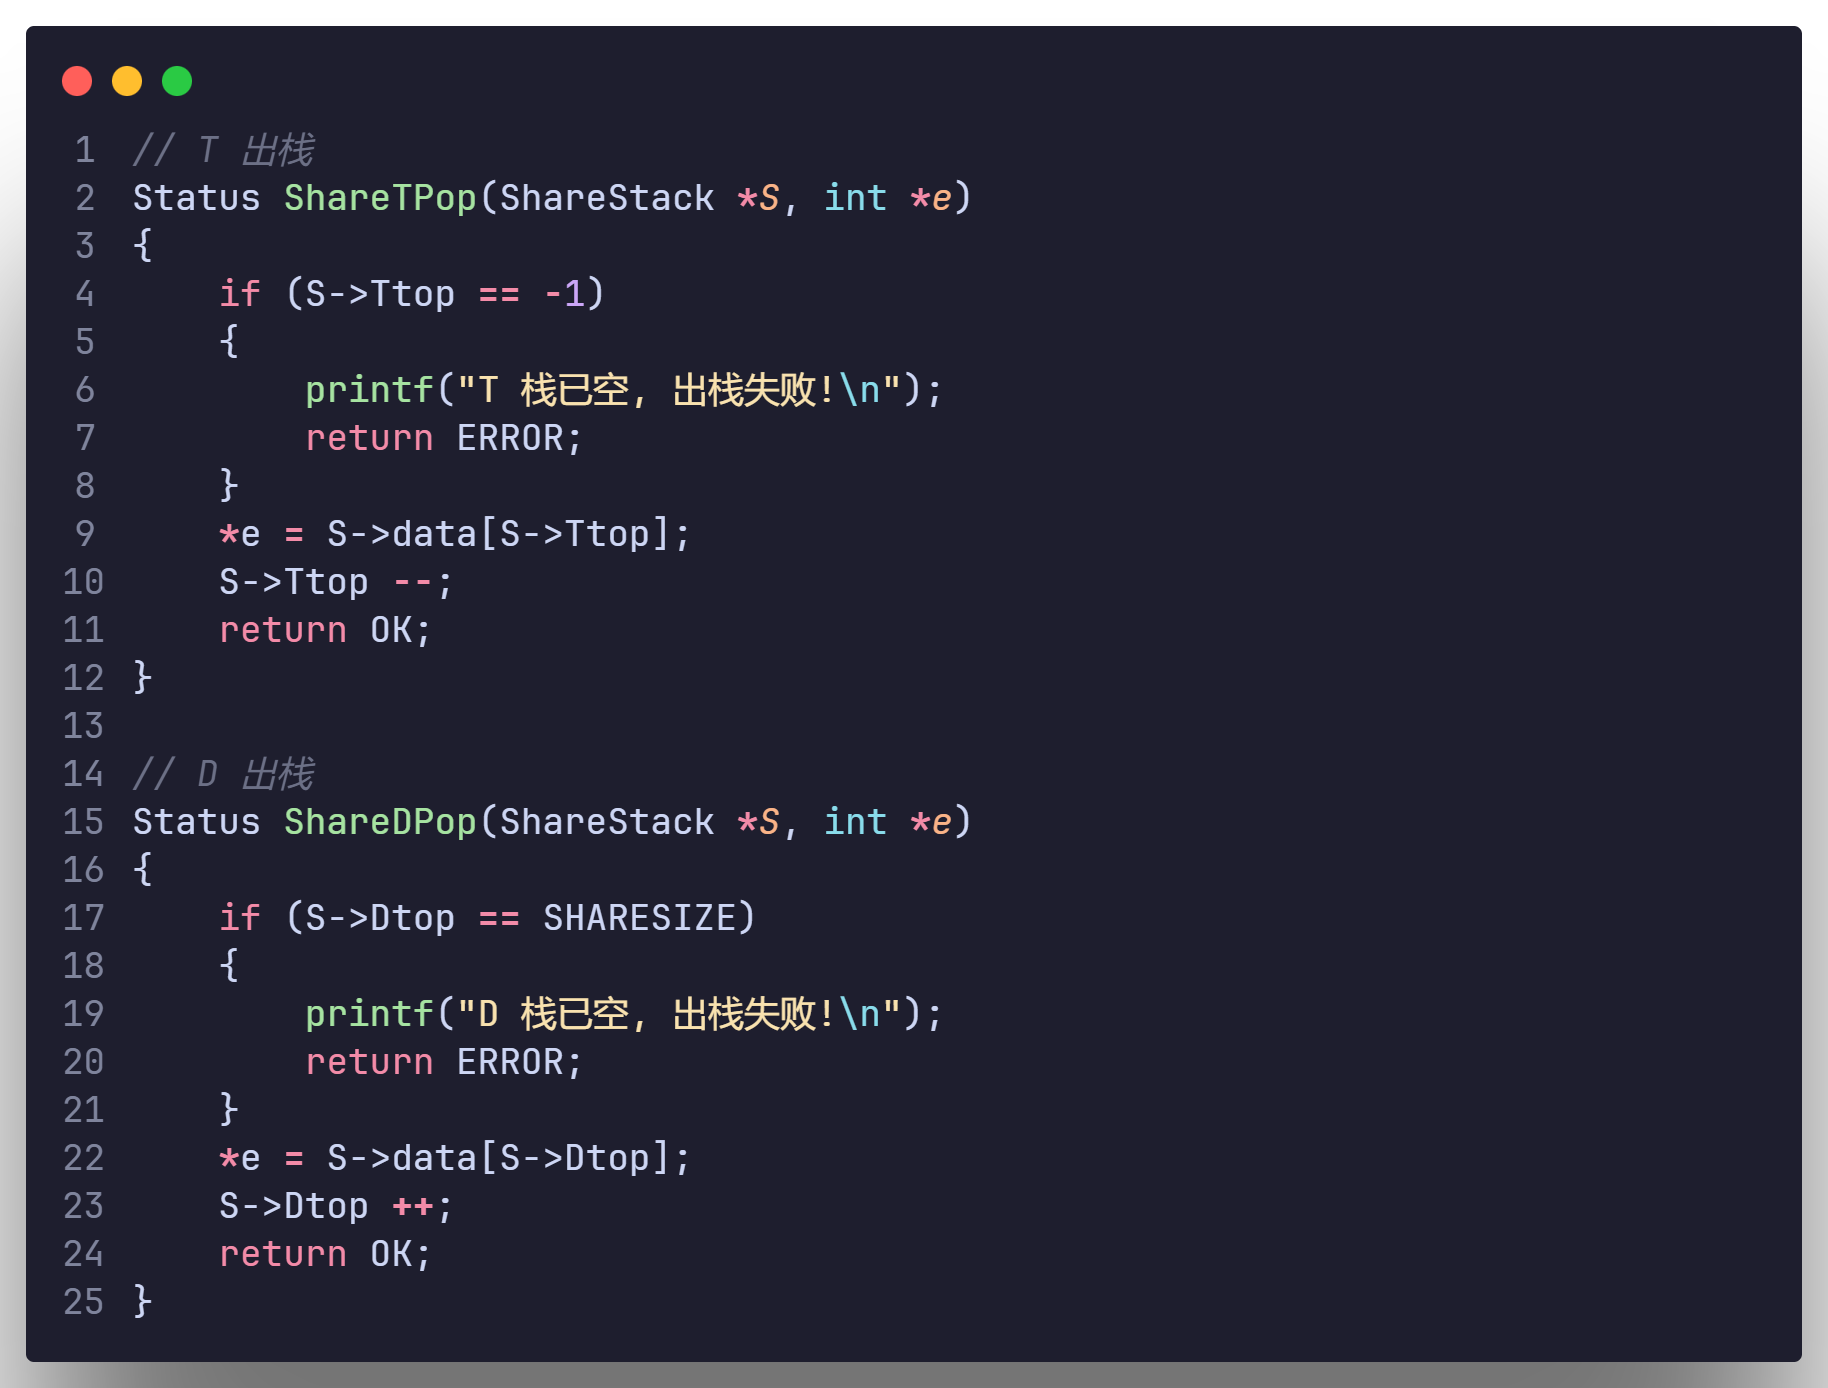
\includegraphics[scale=0.2]{"figure/Note/Stack/SSPop.png"}
\end{figure}

\subsubsection{共享栈辅助函数}

(1). 判断栈是否为空

\begin{figure}[H]
    \centering
    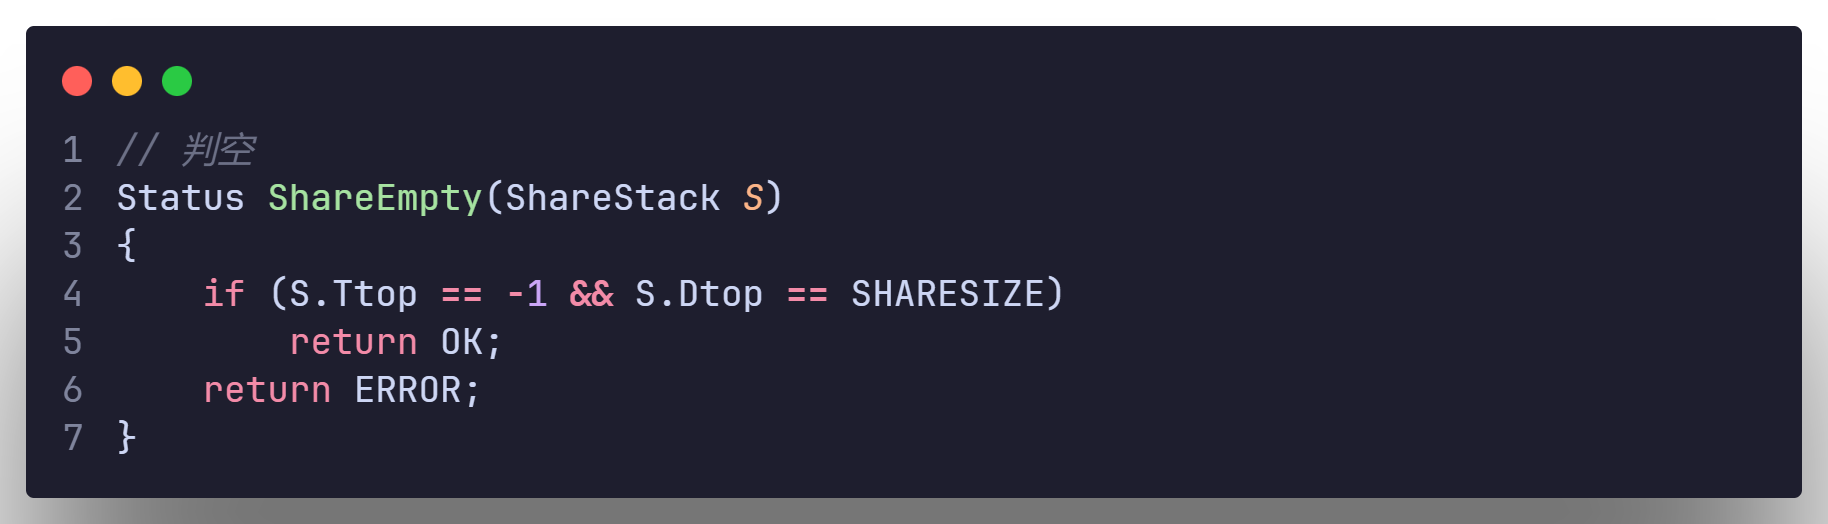
\includegraphics[scale=0.2]{"figure/Note/Stack/SSEmpty.png"}
\end{figure}

(2). 获取栈顶元素

\begin{figure}[H]
    \centering
    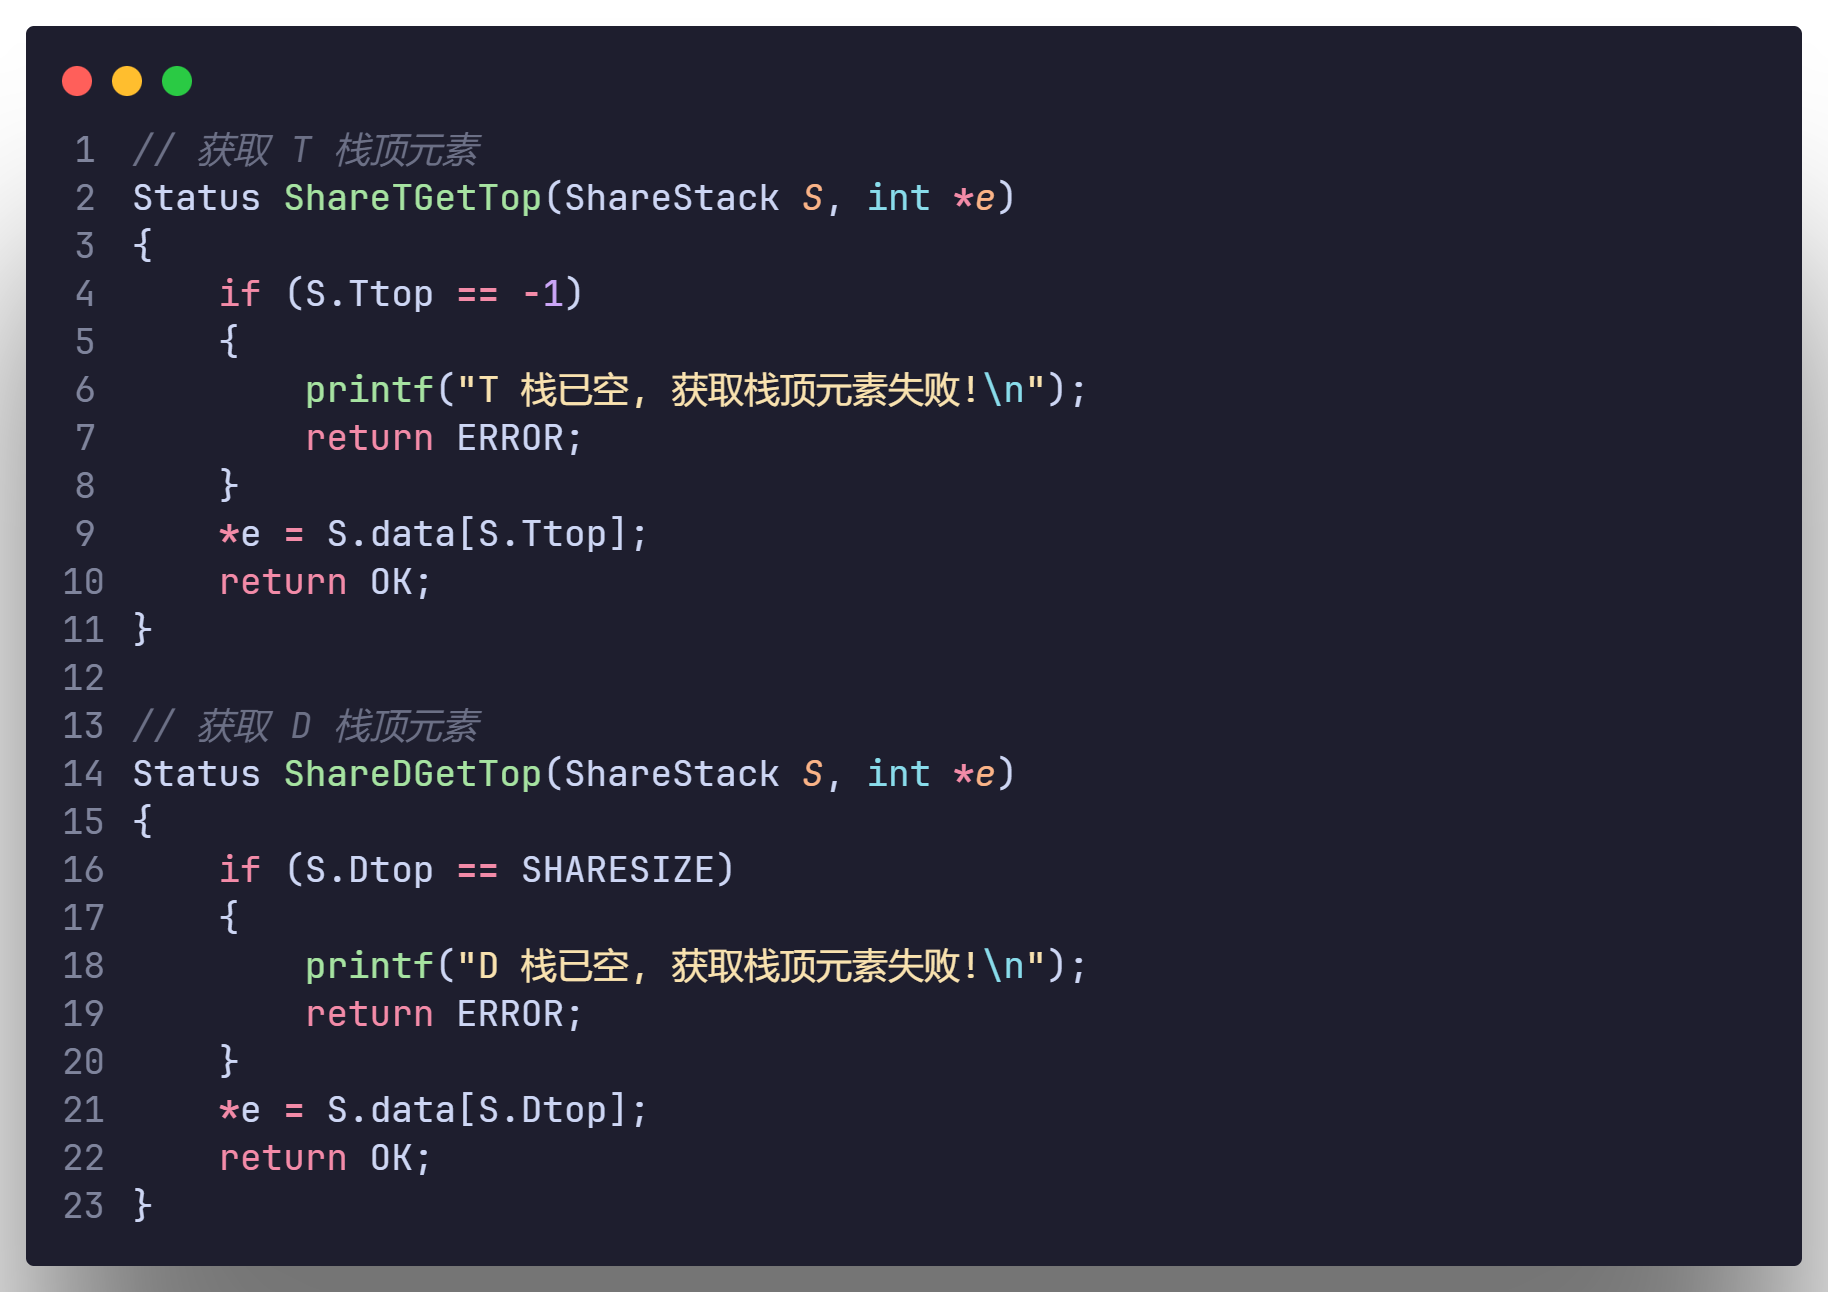
\includegraphics[scale=0.2]{"figure/Note/Stack/SSG.png"}
\end{figure}

(3). 获取栈中元素个数

\begin{figure}[H]
    \centering
    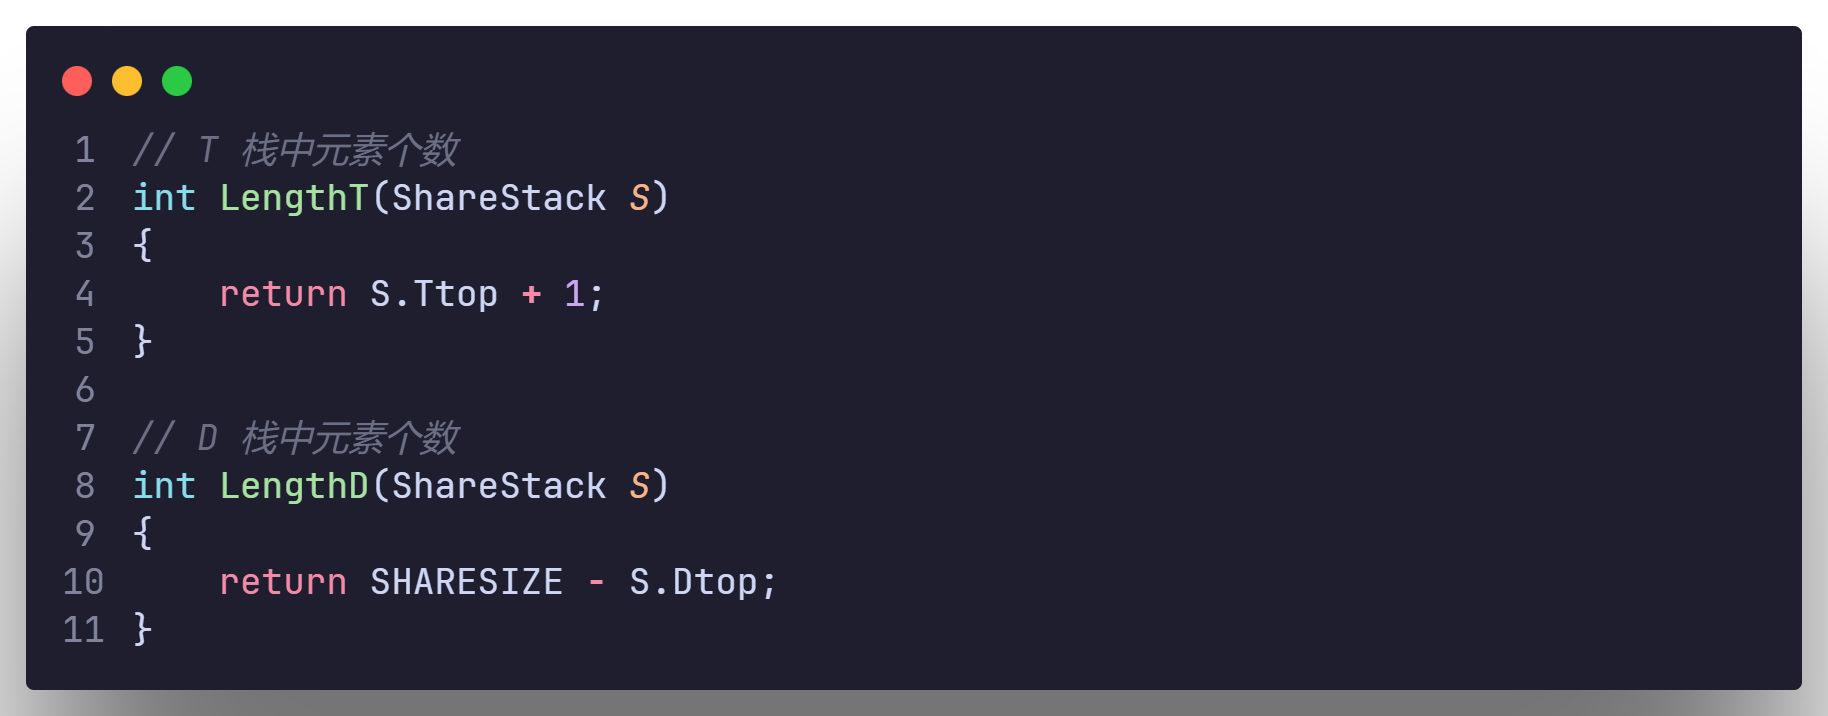
\includegraphics[scale=0.2]{"figure/Note/Stack/SSN.png"}
\end{figure}

(4). 打印栈中元素

\begin{figure}[H]
    \centering
    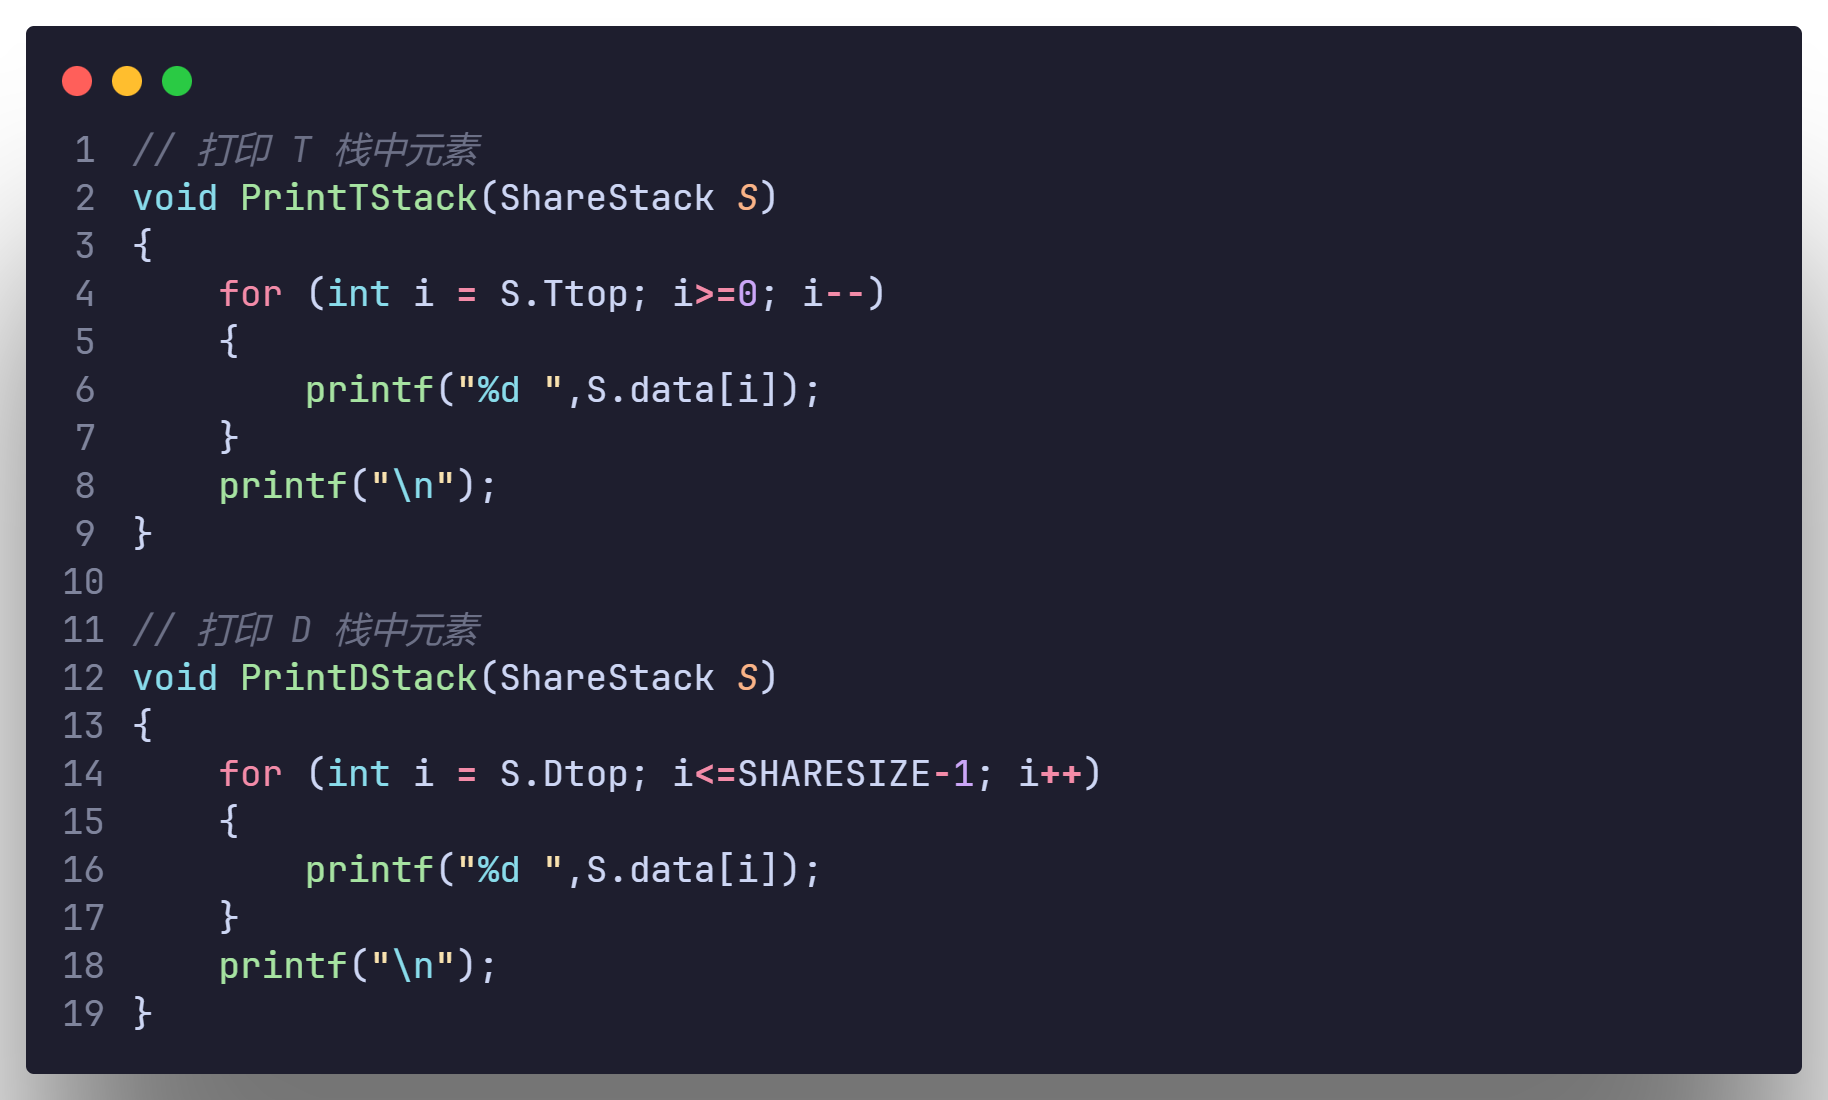
\includegraphics[scale=0.2]{"figure/Note/Stack/SSPrint.png"}
\end{figure}


\section{队列}
\begin{definition}[队列]
    \begin{enumerate}
        \item 只允许在一端进行插入操作,在另一端进行删除操作的线性表
        \item 队列有队头、队尾两个重要元素,队头元素是最先插入的元素,队尾元素是最后插入的元素
        \item 队列的插入操作叫做入队,队列的删除操作叫做出队
        \item 队列的特点是先进先出,简称 $\mathbf{FIFO}, \mathbf{First\ In\ First\ Out}$
    \end{enumerate}
\end{definition}
\begin{definition}[特殊队列]
    1. 循环队列: 顺序表实现的队列,解决顺序表的假溢出问题

    2. 双端队列: 两端都可以进行插入和删除操作的队列

    3. 操作受限的双端队列: 两端都可以进行插入和删除操作,但是有限制,比如只有一端可以插入或者删除
\end{definition}

\begin{definition}[队列基本操作]
    \begin{enumerate}
        \item $\mathbf{InitQueue(\& Q)}$  初始化队列 $Q$
        \item $\mathbf{DestroyQueue(\& Q)}$  销毁队列 $Q$
        \item $\mathbf{GetHead(Q,\&e)}$ 获取队首元素,将队列 $Q$ 队首元素赋值给 $e$
        \item $\mathbf{EnQueue(\&S,e)}$ 入队
        \item $\mathbf{DeQueue(\&S,\&e)}$ 出队
        \item $\mathbf{Length(Q)}$ 求队列中元素个数
        \item $\mathbf{Empty(Q)}$ 判空
        \item $\mathbf{PrintQueue(S)}$ 输出操作,输出队列 $Q$ 的所有元素 
    \end{enumerate}
\end{definition}
\subsection{队列定义和函数声明}
\subsubsection{循环队列、链表队列定义}

\begin{figure}[H]
    \centering
    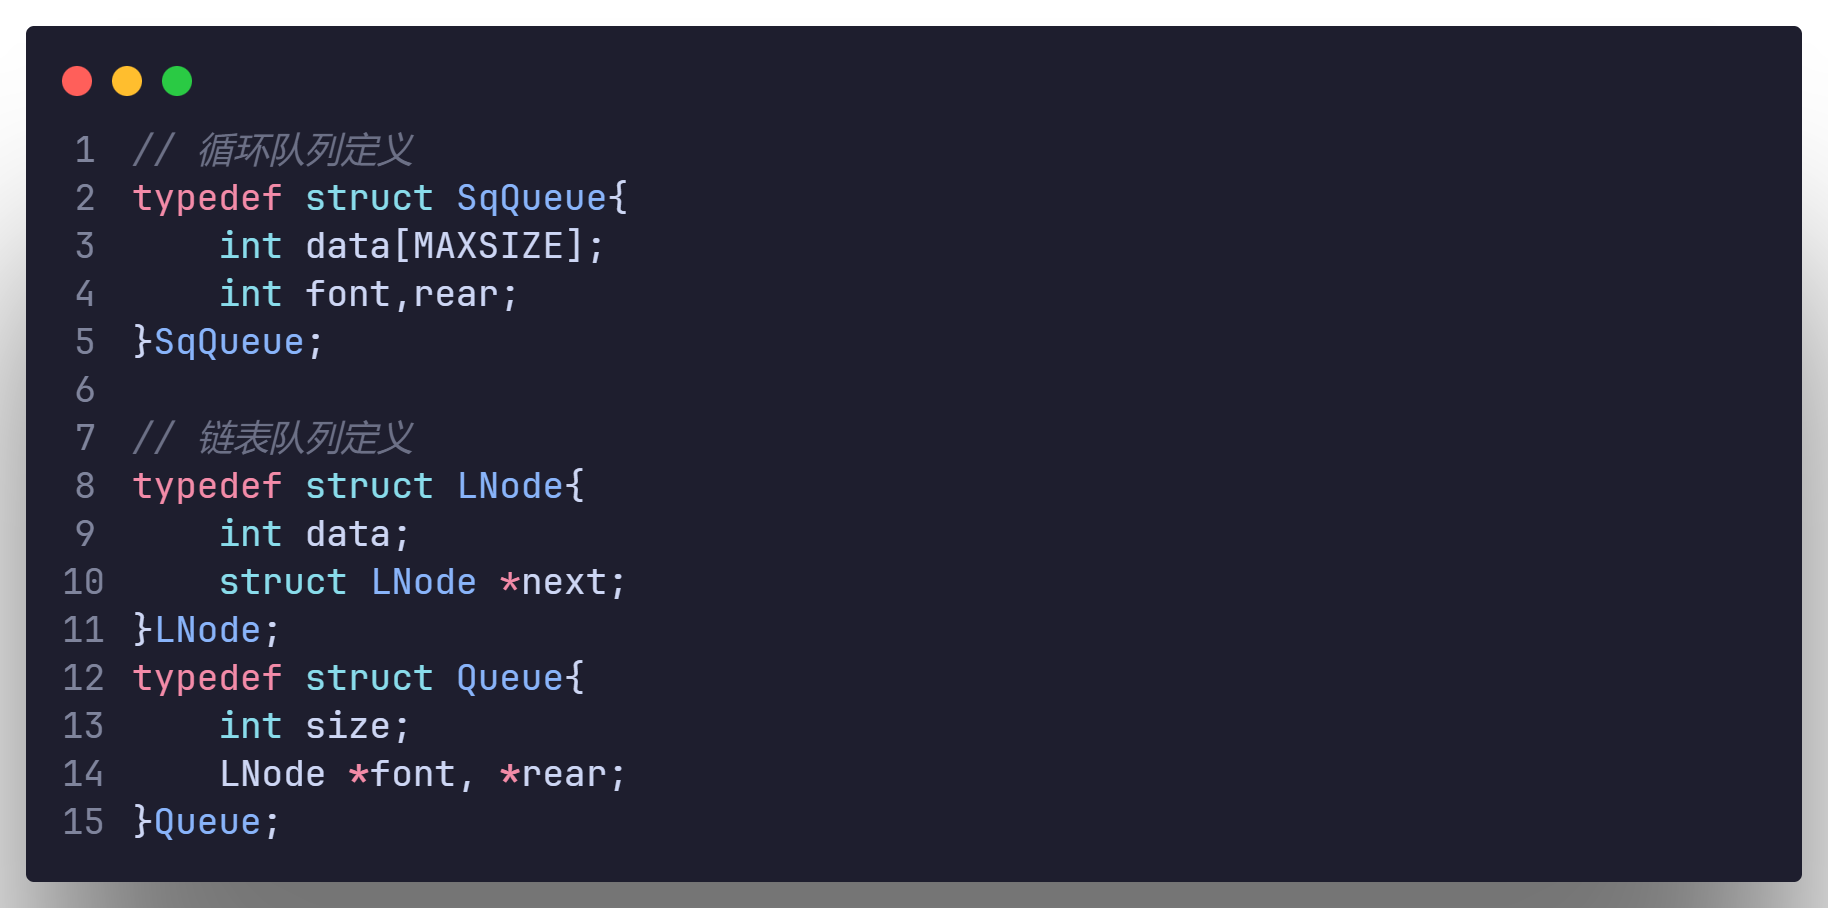
\includegraphics[scale=0.2]{"figure/Note/Stack/QDefine.png"}
\end{figure}

\subsubsection{函数声明}

\begin{figure}[H]
    \centering
    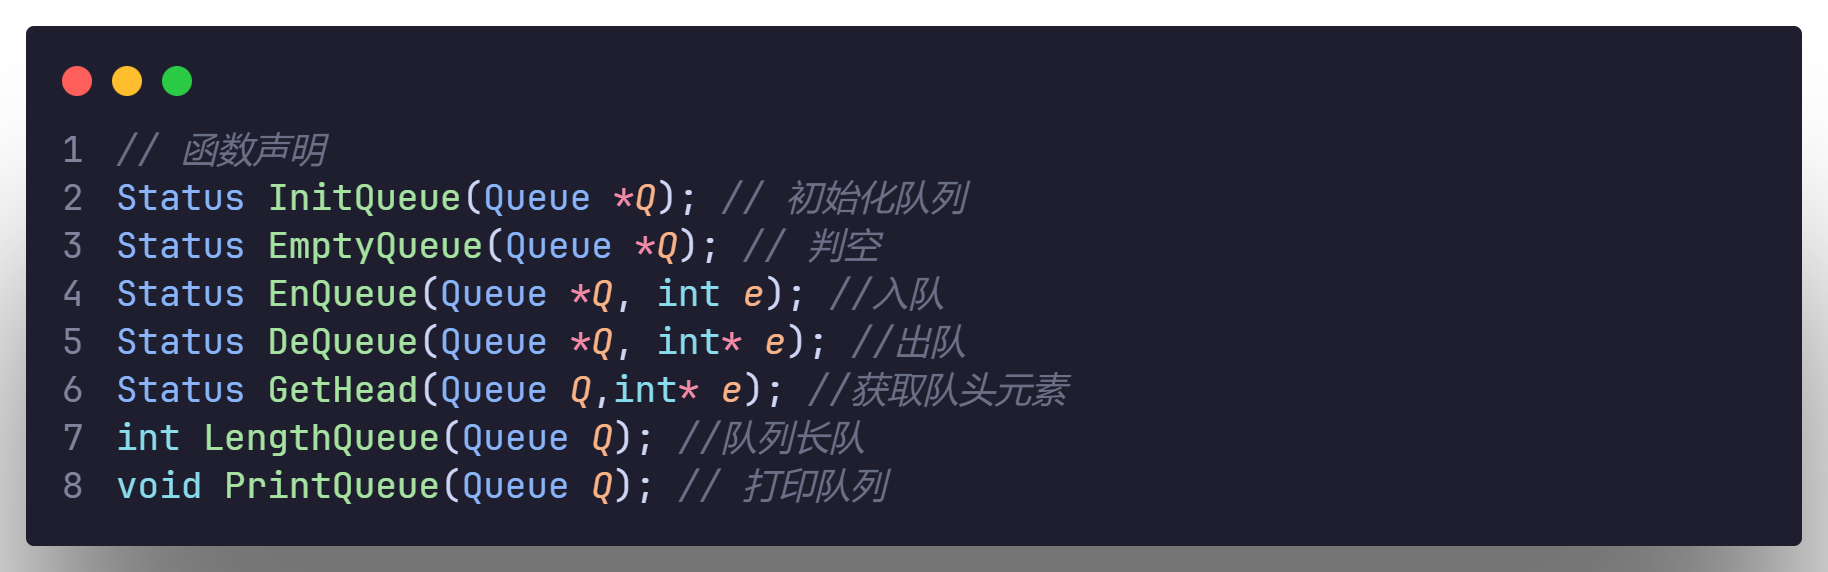
\includegraphics[scale=0.2]{"figure/Note/Stack/QFunction.png"}
\end{figure}

\subsection{循环队列}
\begin{definition}[循环队列]
    循环队列是使用顺序表实现的队列,为防止出现假溢出,将顺序表的首尾相连,当队尾指针指向顺序表的最后一个位置时,再插入元素时,将队尾指针指向顺序表的第一个位置.

    \textbf{实现方法:}
    \begin{enumerate}
        \item 队列最后一个位置不存储元素,队列中元素个数最多为 $MAXSIZE-1$, 队列满的条件是 $(Q.rear+1)\% MAXSIZE == Q.font$, 队列空的条件是 $Q.rear == Q.font$
        \item 设置一个标志位 $\mathbf{flag}$, 如果 $flag = 0$, 表示上一次是入队操作, 如果 $flag = 1$, 表示上一次是出队操作, 当 $Q.rear == Q.font$ 时, 根据 $flag$ 的值判断是队列满还是队列空, 如果 $flag = 0$, 队列满, 如果 $flag = 1$, 队列空
    \end{enumerate}
\end{definition}
\subsubsection{循环队列初始化}

\begin{figure}[H]
    \centering
    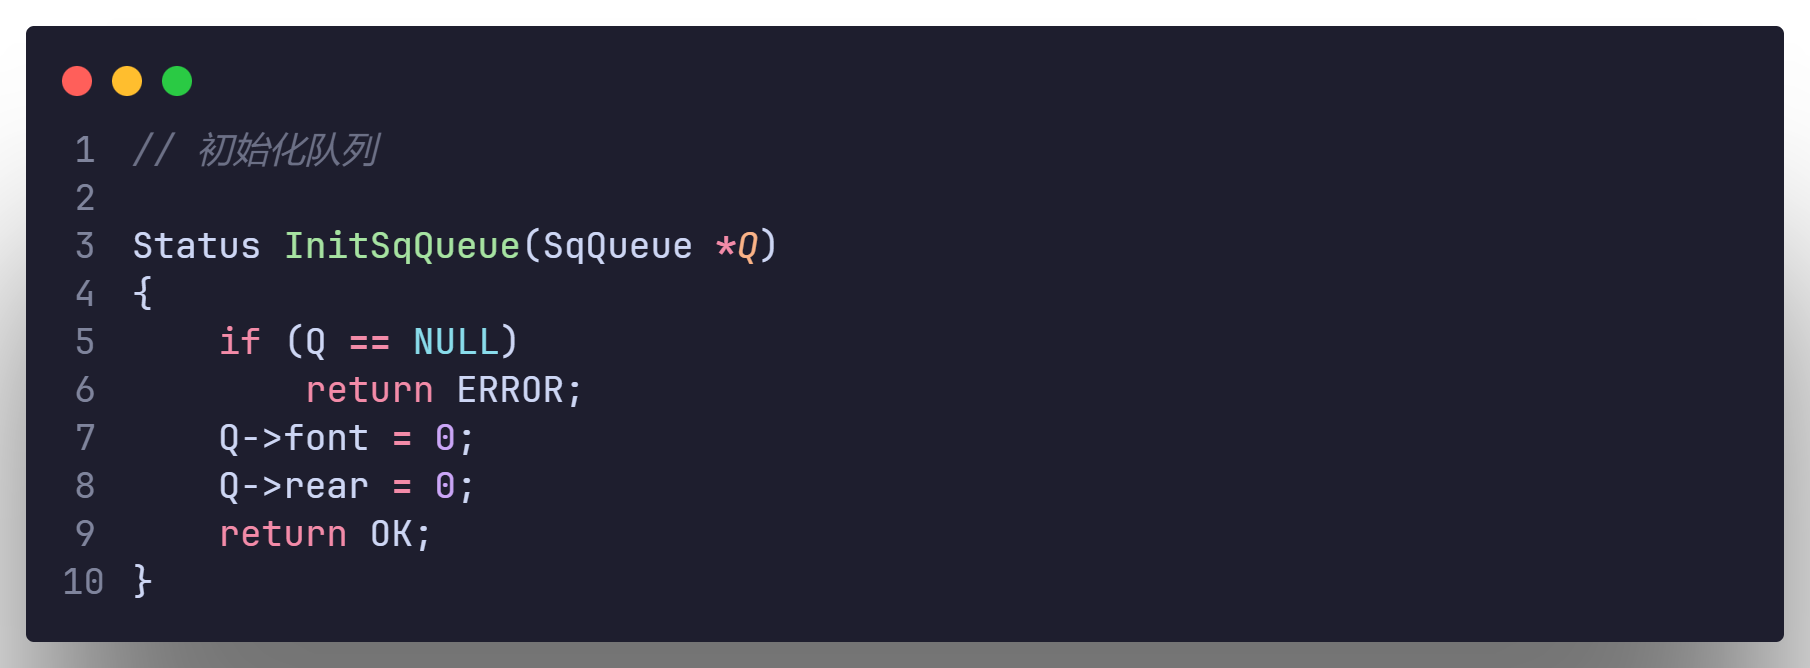
\includegraphics[scale=0.2]{"figure/Note/Stack/QInit.png"}
\end{figure}

\subsubsection{循环队列出入队}

(1). 入队

\begin{figure}[H]
    \centering
    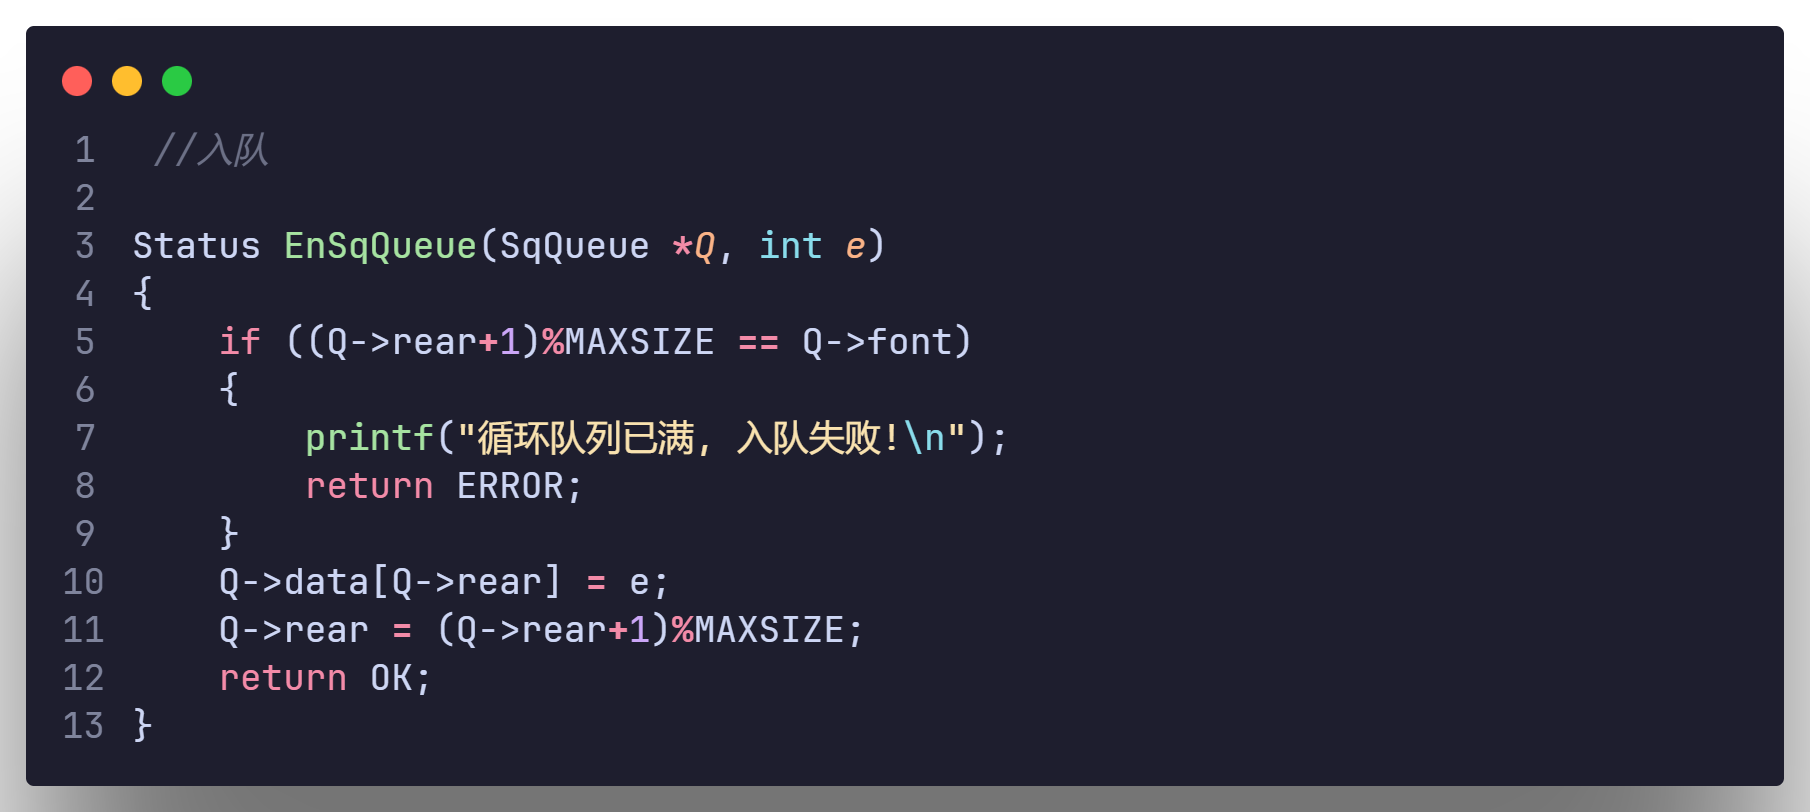
\includegraphics[scale=0.2]{"figure/Note/Stack/QEq.png"}
\end{figure}

(2). 出队

\begin{figure}[H]
    \centering
    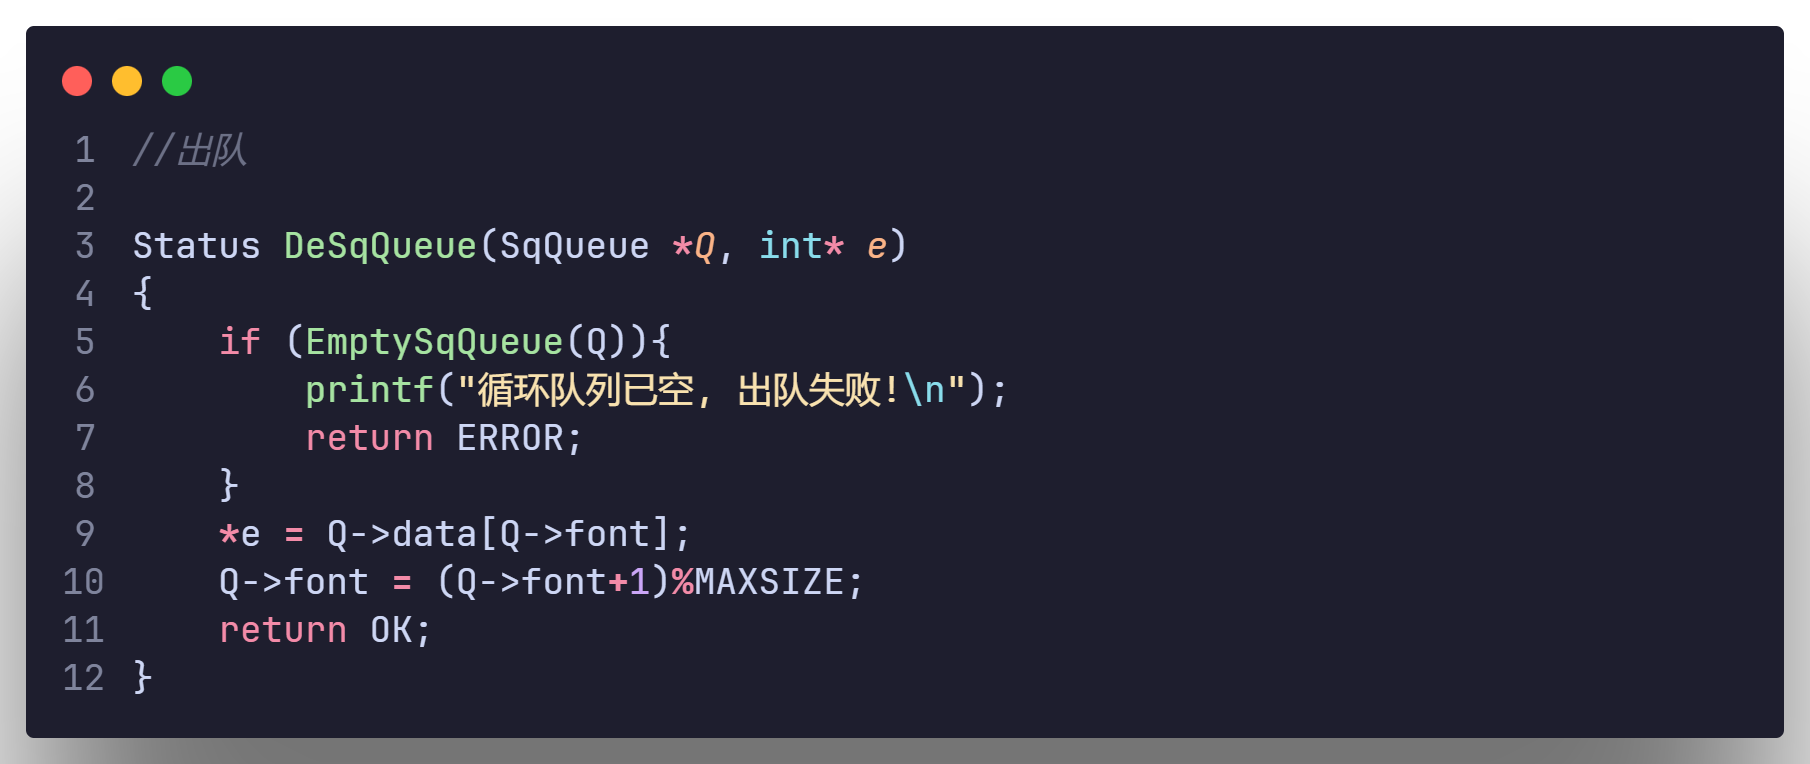
\includegraphics[scale=0.2]{"figure/Note/Stack/QDq.png"}
\end{figure}

\subsubsection{循环队列辅助函数}
(1). 获取队首元素

\begin{figure}[H]
    \centering
    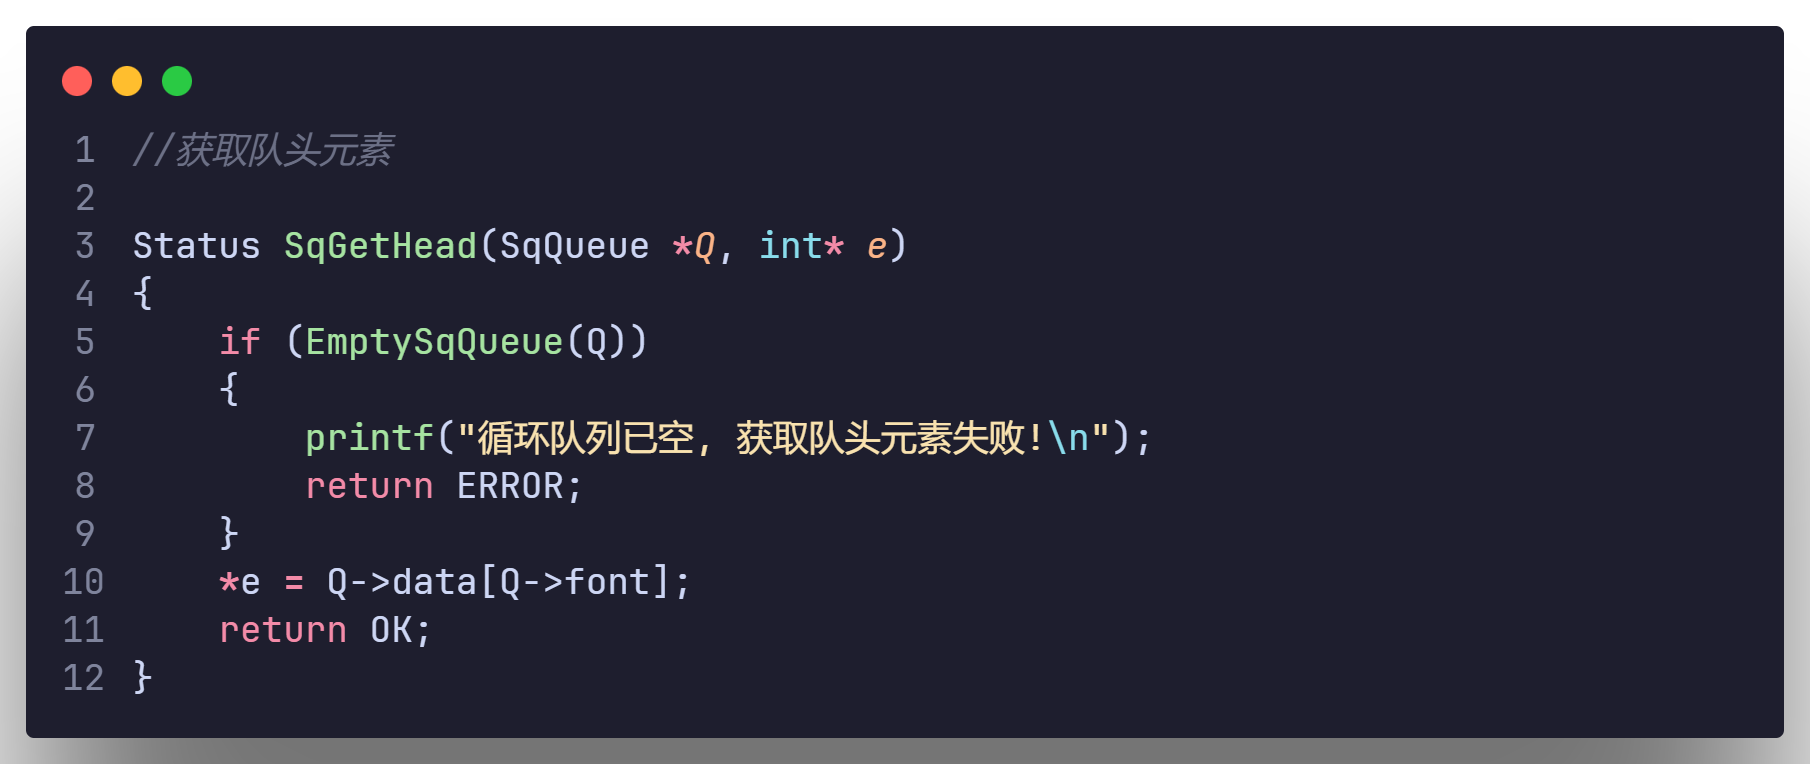
\includegraphics[scale=0.2]{"figure/Note/Stack/QG.png"}
\end{figure}

(2). 队列长度

\begin{figure}[H]
    \centering
    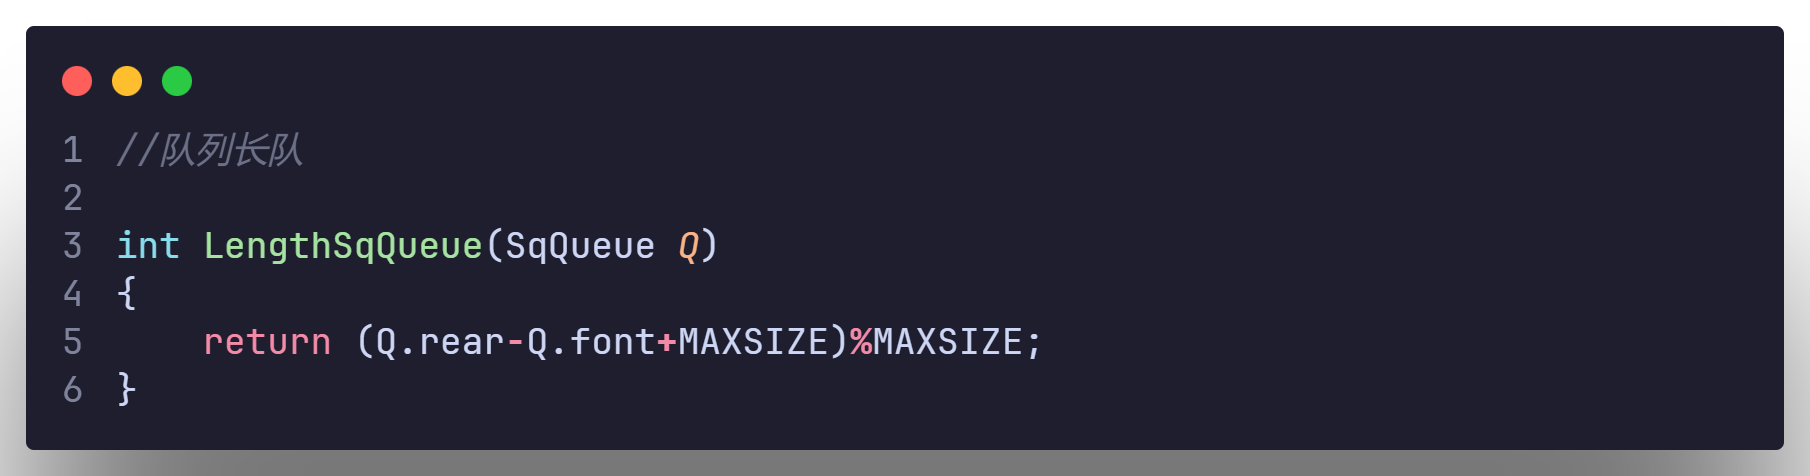
\includegraphics[scale=0.2]{"figure/Note/Stack/QLen.png"}
\end{figure}

(3). 判断队列是否为空

\begin{figure}[H]
    \centering
    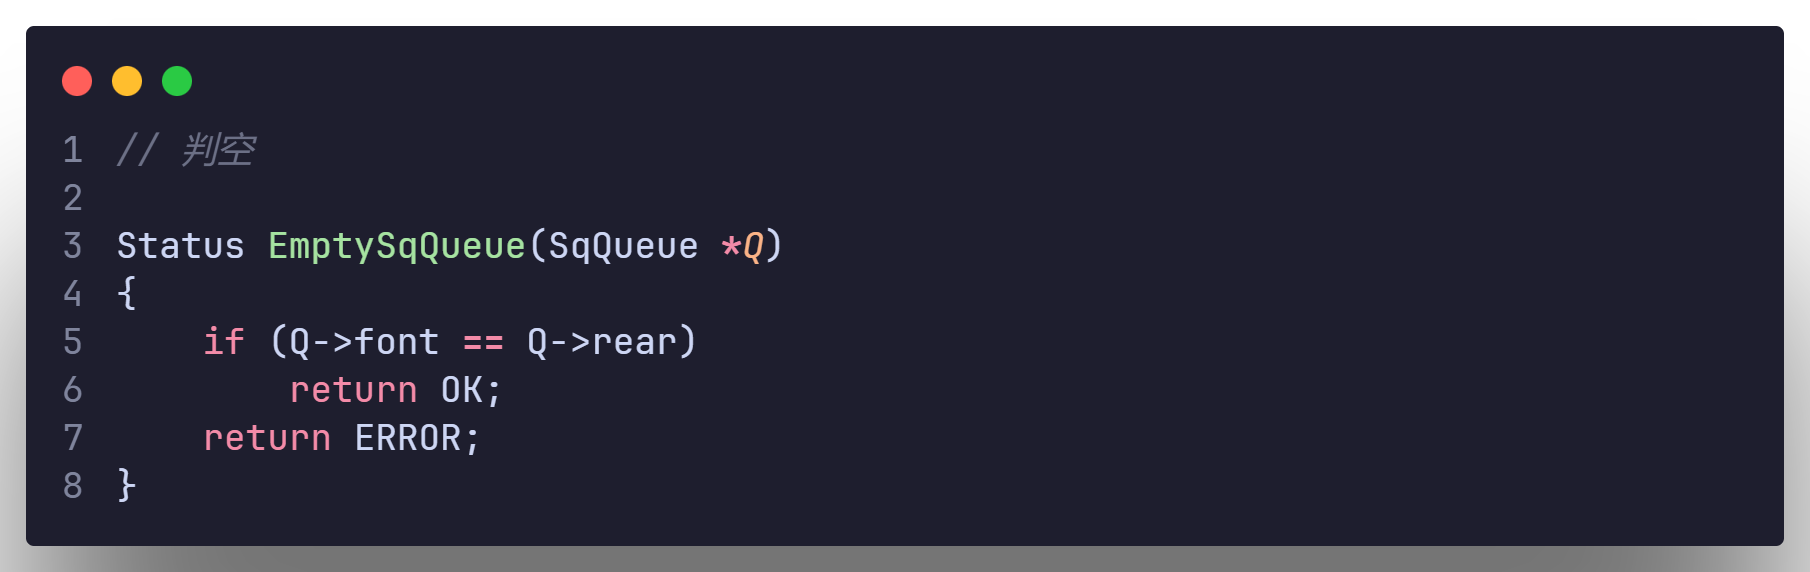
\includegraphics[scale=0.2]{"figure/Note/Stack/QEmpty.png"}
\end{figure}

(4). 打印队列

\begin{figure}[H]
    \centering
    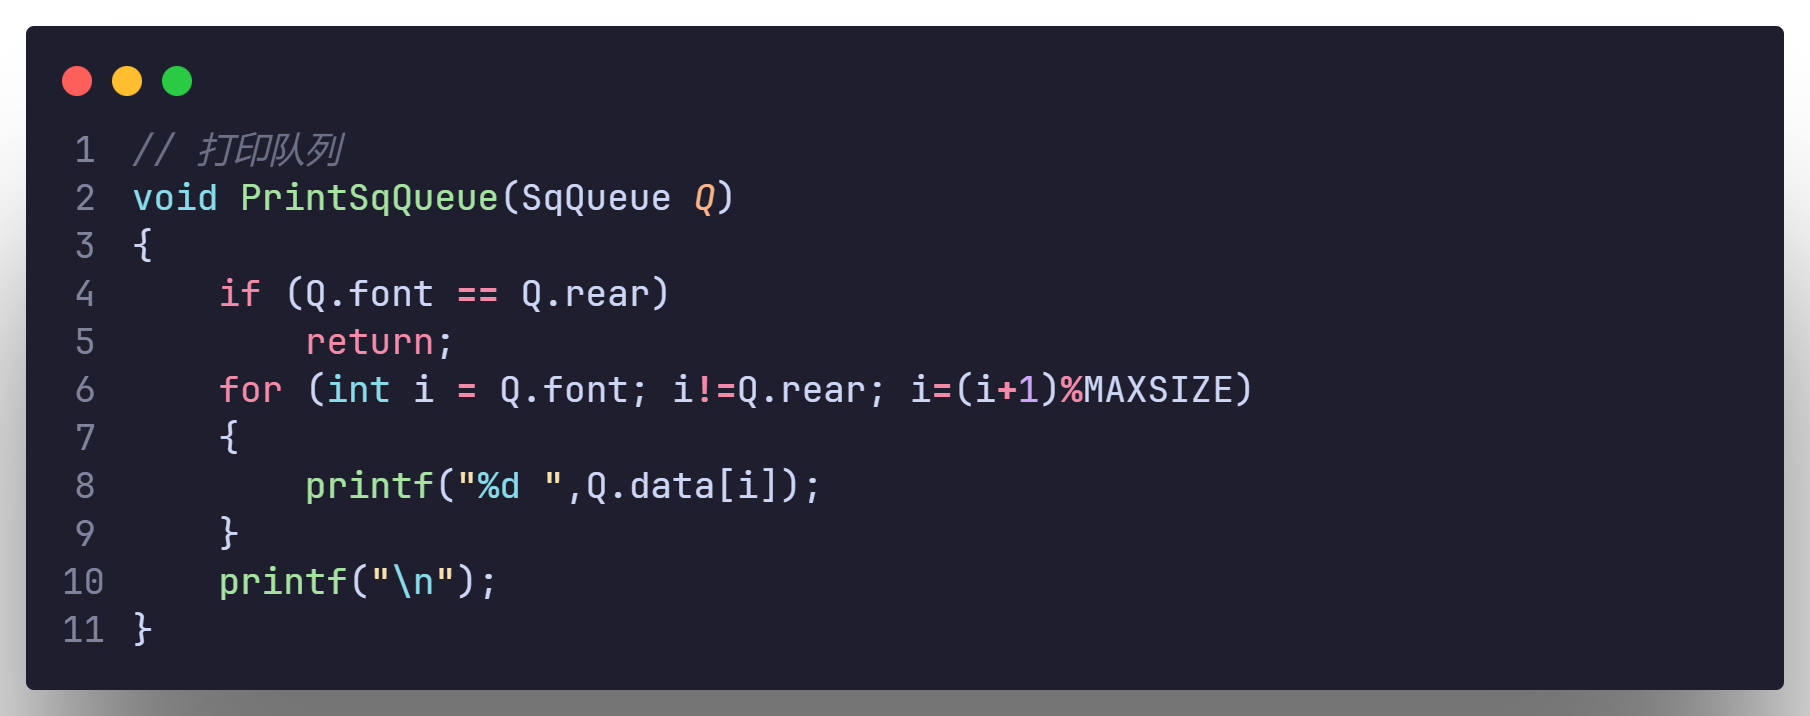
\includegraphics[scale=0.2]{"figure/Note/Stack/QPrint.png"}
\end{figure}

\subsection{链队列}
\begin{definition}[链队列]
    链队列是使用链表实现的队列,只需要存储队头节点和队尾节点的指针.

    \textbf{实现方法:}
    \begin{enumerate}
        \item 队列入队, 将新节点作为队尾节点的后继节点, 队尾节点变为新节点
        \item 队列出队, 将队头节点作为出队节点, 队头节点变为其后继节点, 释放队头节点的空间
    \end{enumerate}
\end{definition}
\subsubsection{链队列初始化}

\begin{figure}[H]
    \centering
    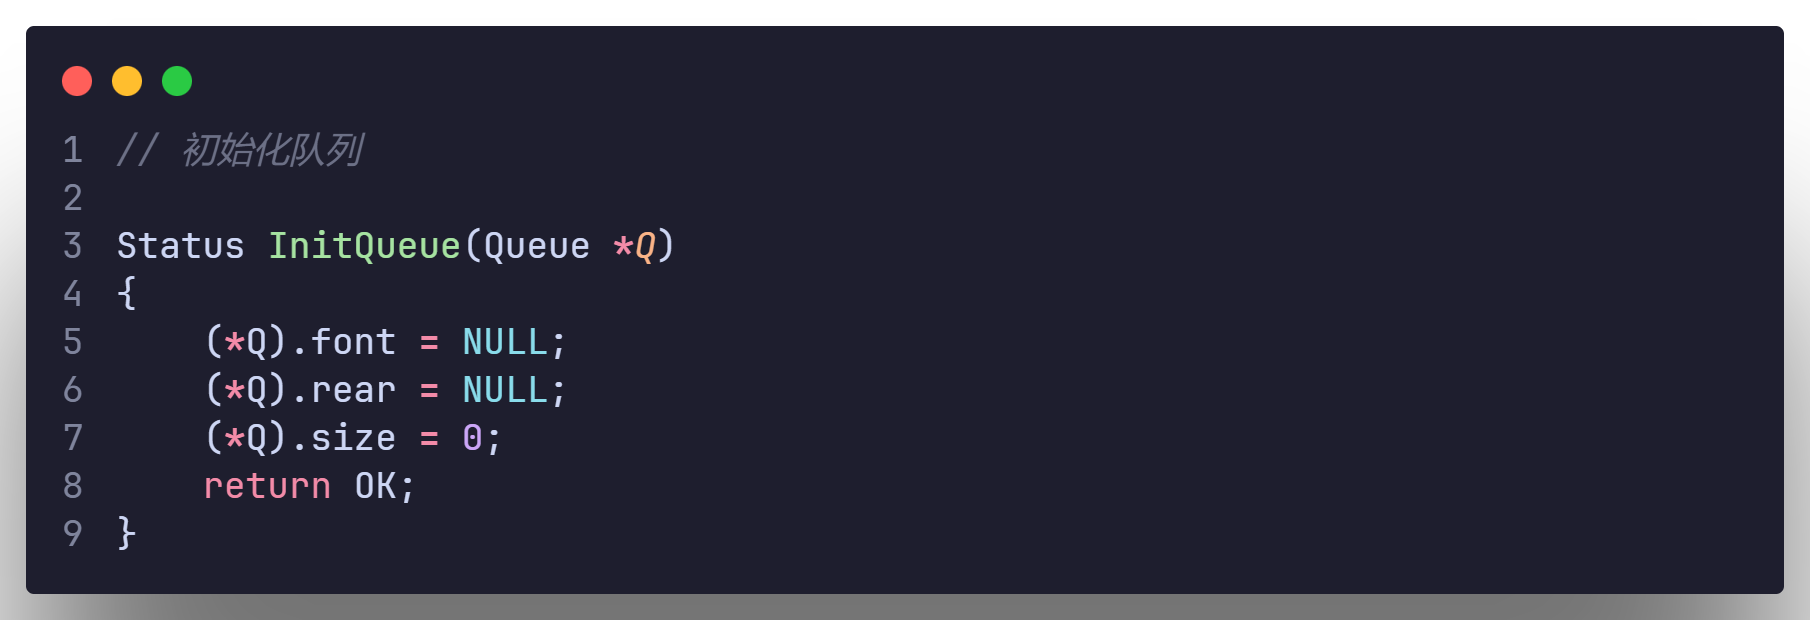
\includegraphics[scale=0.2]{"figure/Note/Stack/QlInit.png"}
\end{figure}

\subsubsection{链队列出入队}

(1). 入队

\begin{figure}[H]
    \centering
    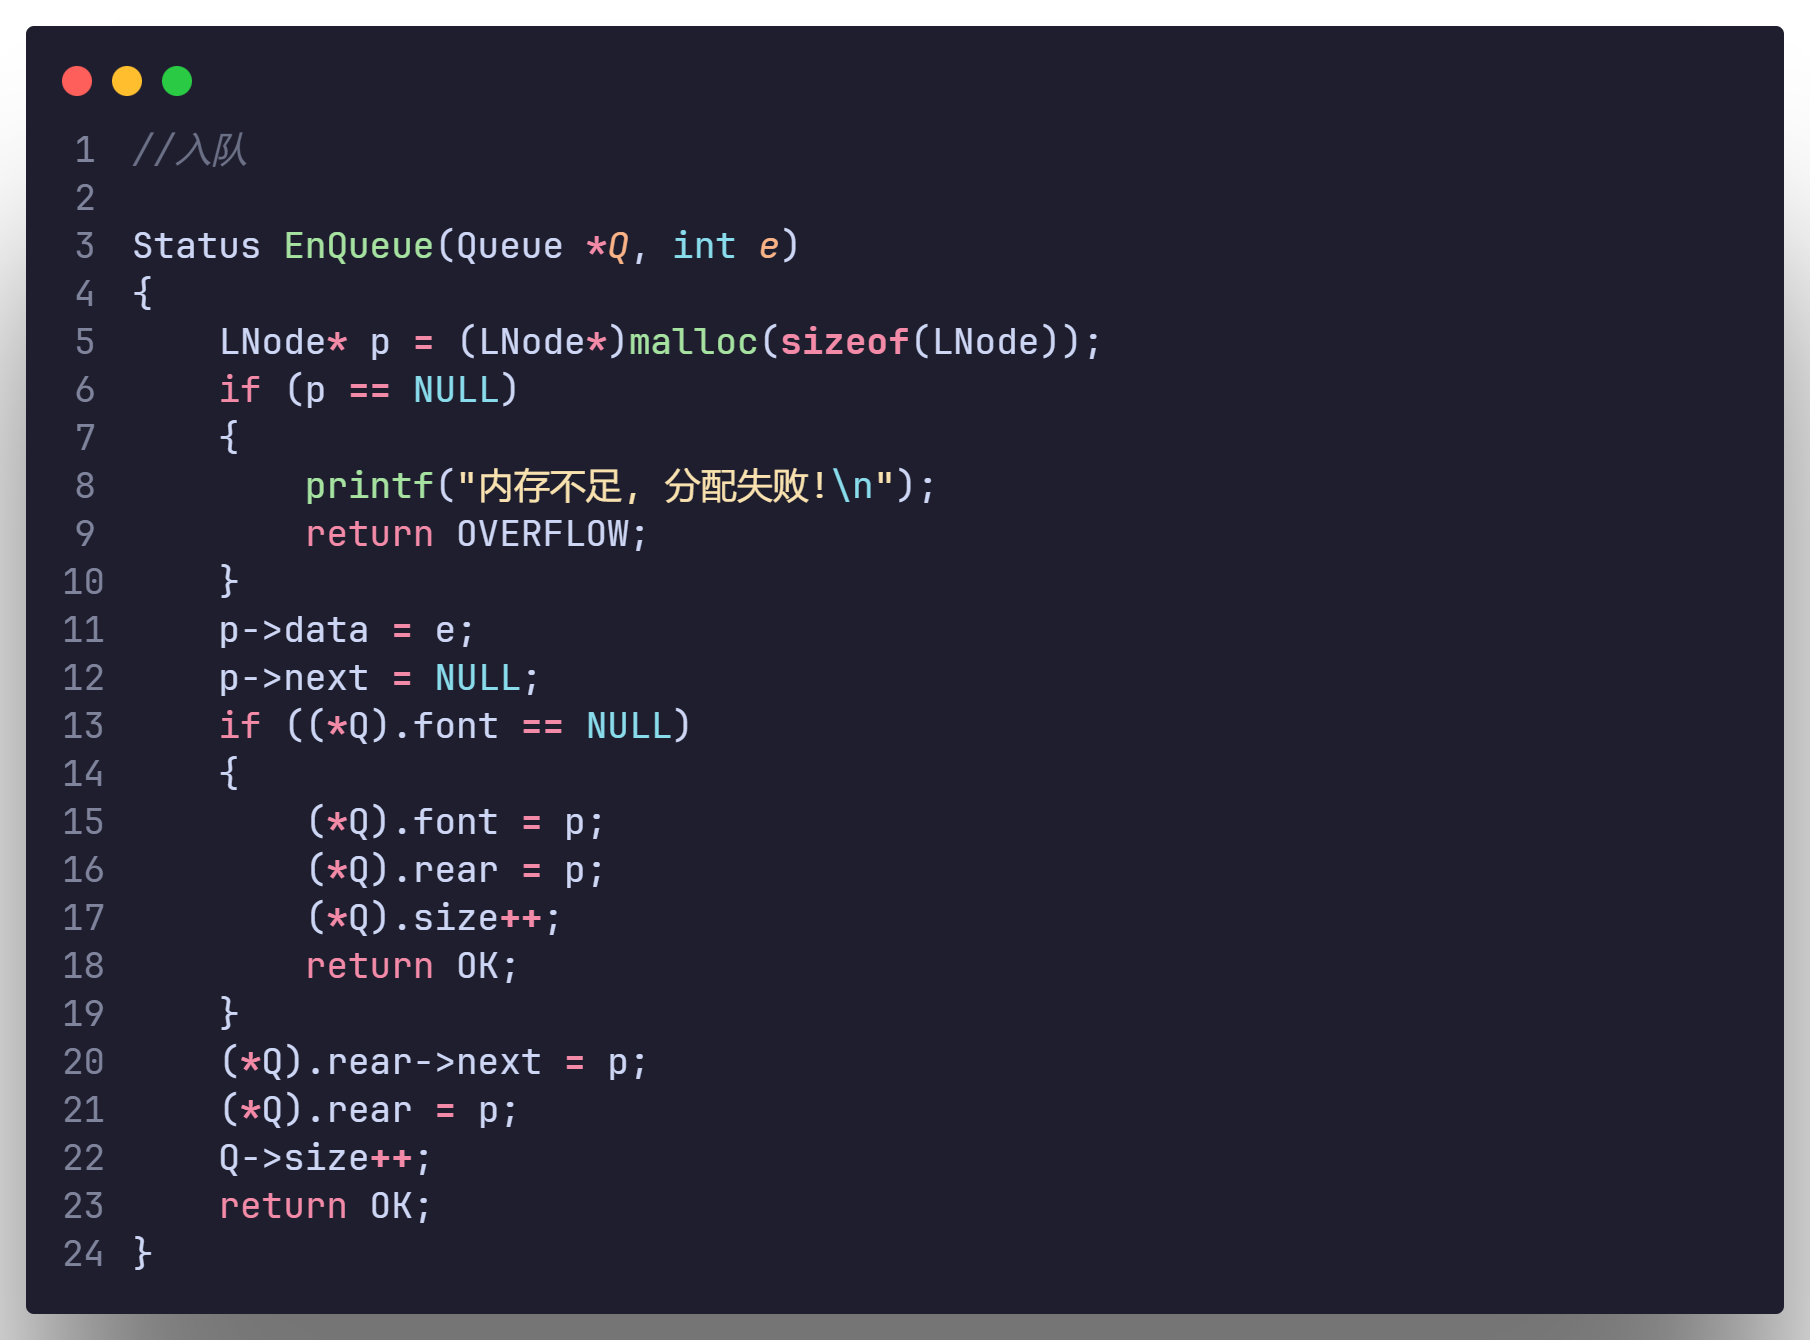
\includegraphics[scale=0.2]{"figure/Note/Stack/QlEq.png"}
\end{figure}

(2). 出队

\begin{figure}[H]
    \centering
    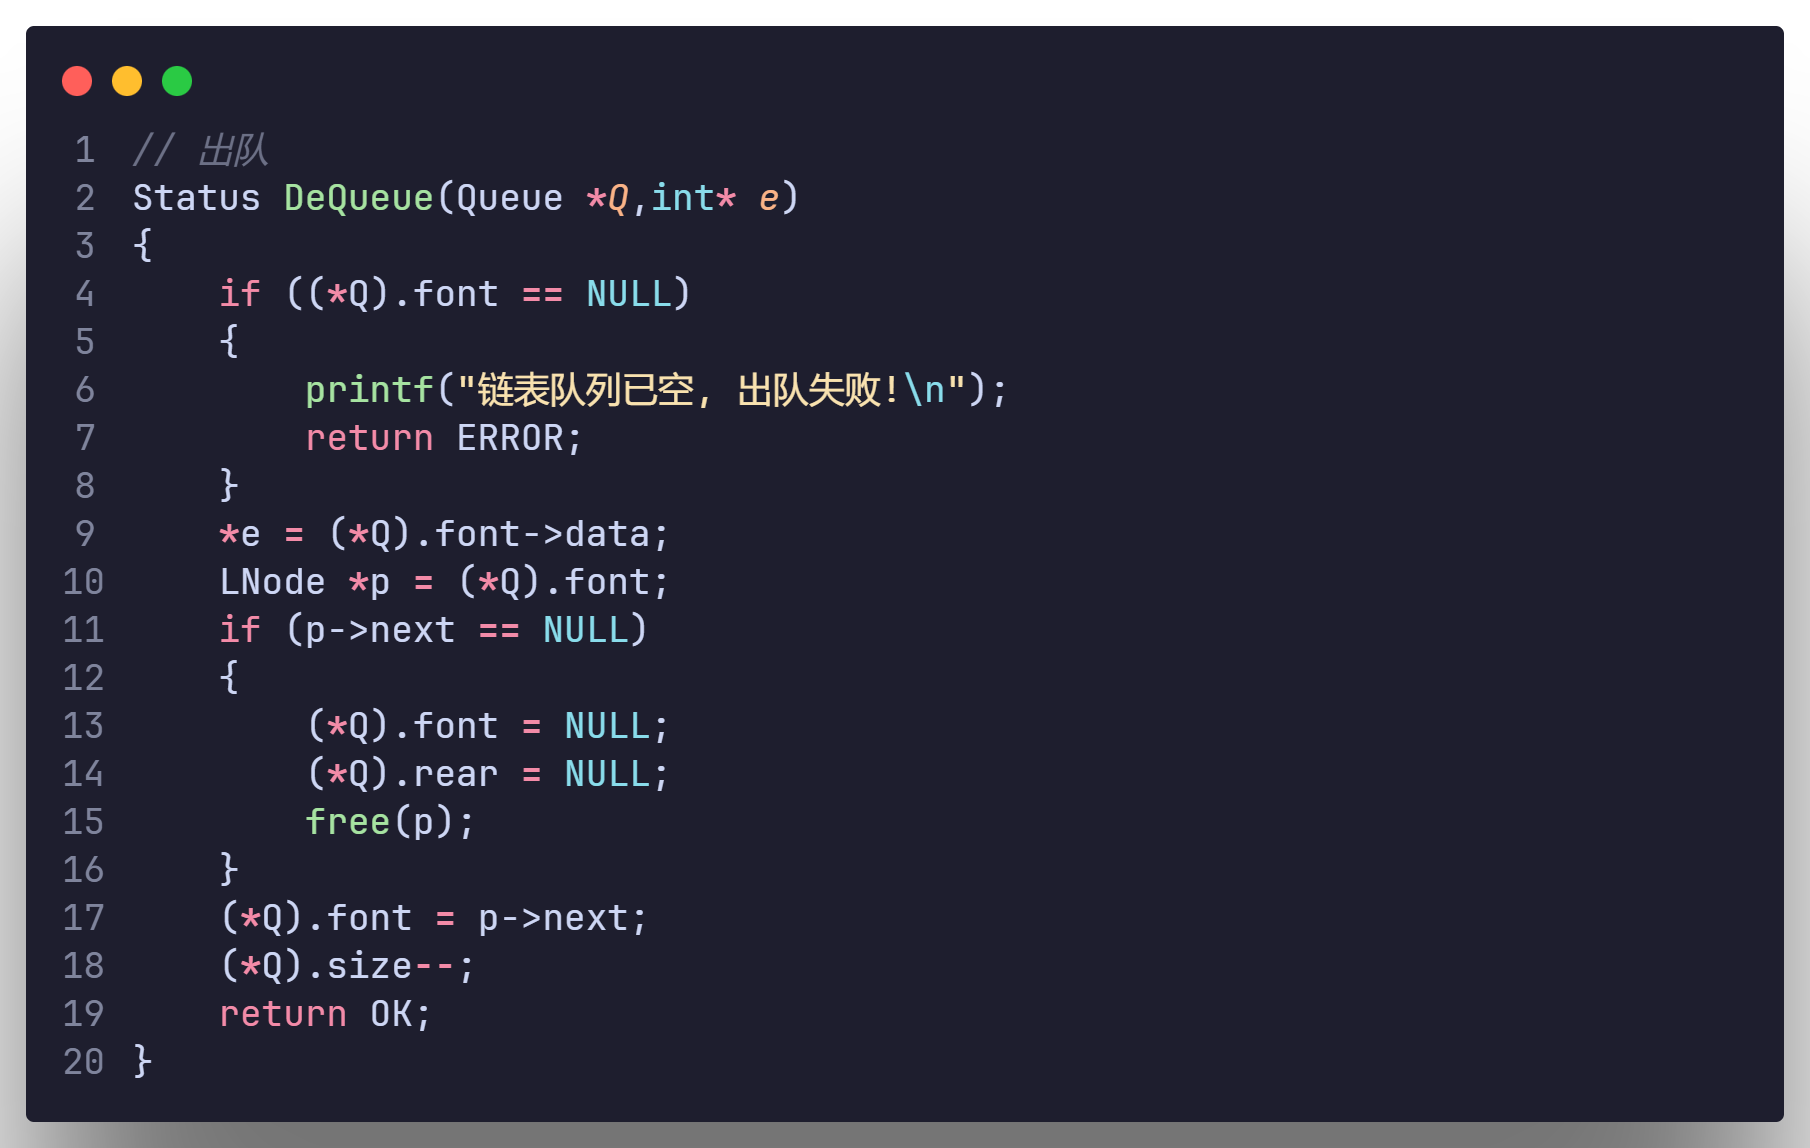
\includegraphics[scale=0.2]{"figure/Note/Stack/QlDq.png"}
\end{figure}

\subsubsection{链队列辅助函数}
(1). 获取队首元素

\begin{figure}[H]
    \centering
    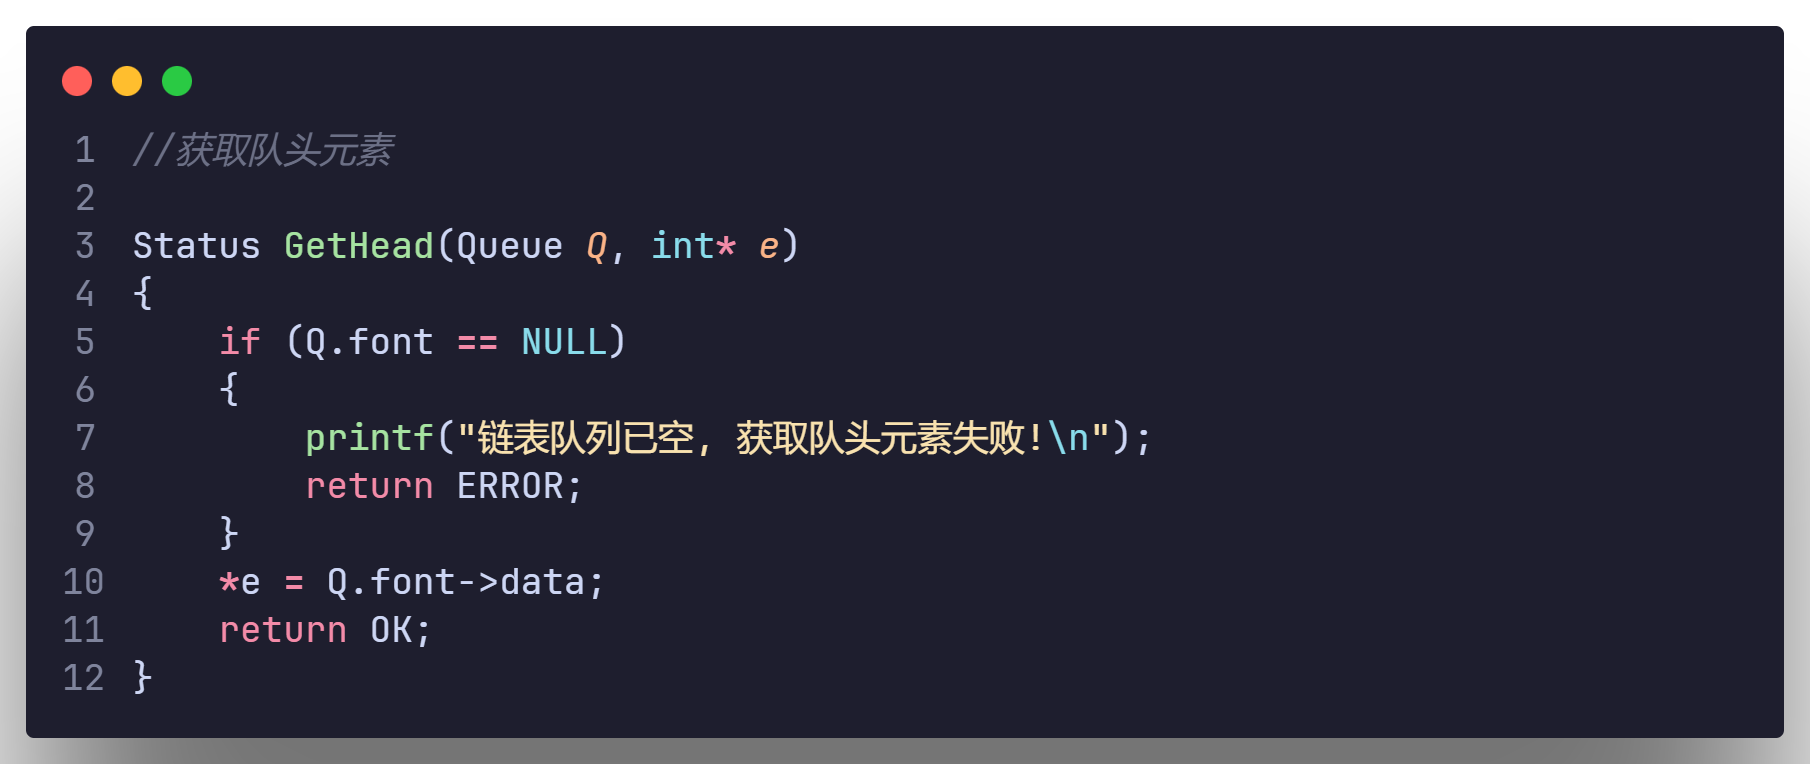
\includegraphics[scale=0.2]{"figure/Note/Stack/QlG.png"}
\end{figure}

(2). 队列长度

\begin{figure}[H]
    \centering
    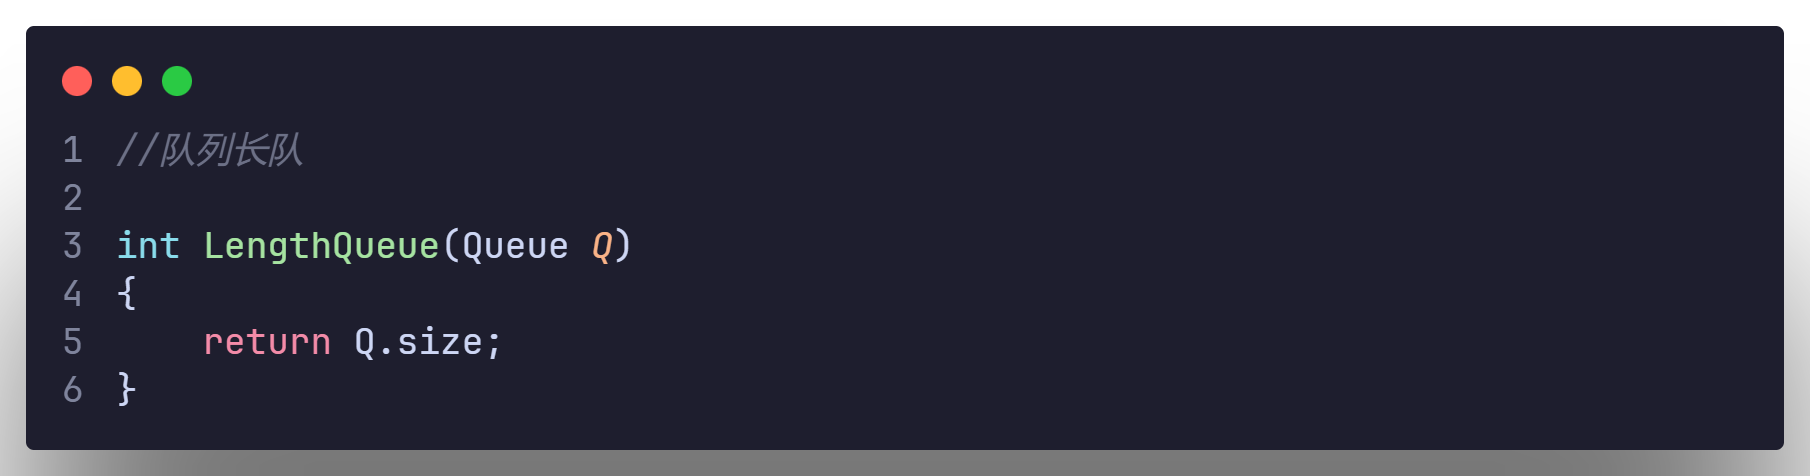
\includegraphics[scale=0.2]{"figure/Note/Stack/QlLen.png"}
\end{figure}

(3). 判断队列是否为空

\begin{figure}[H]
    \centering
    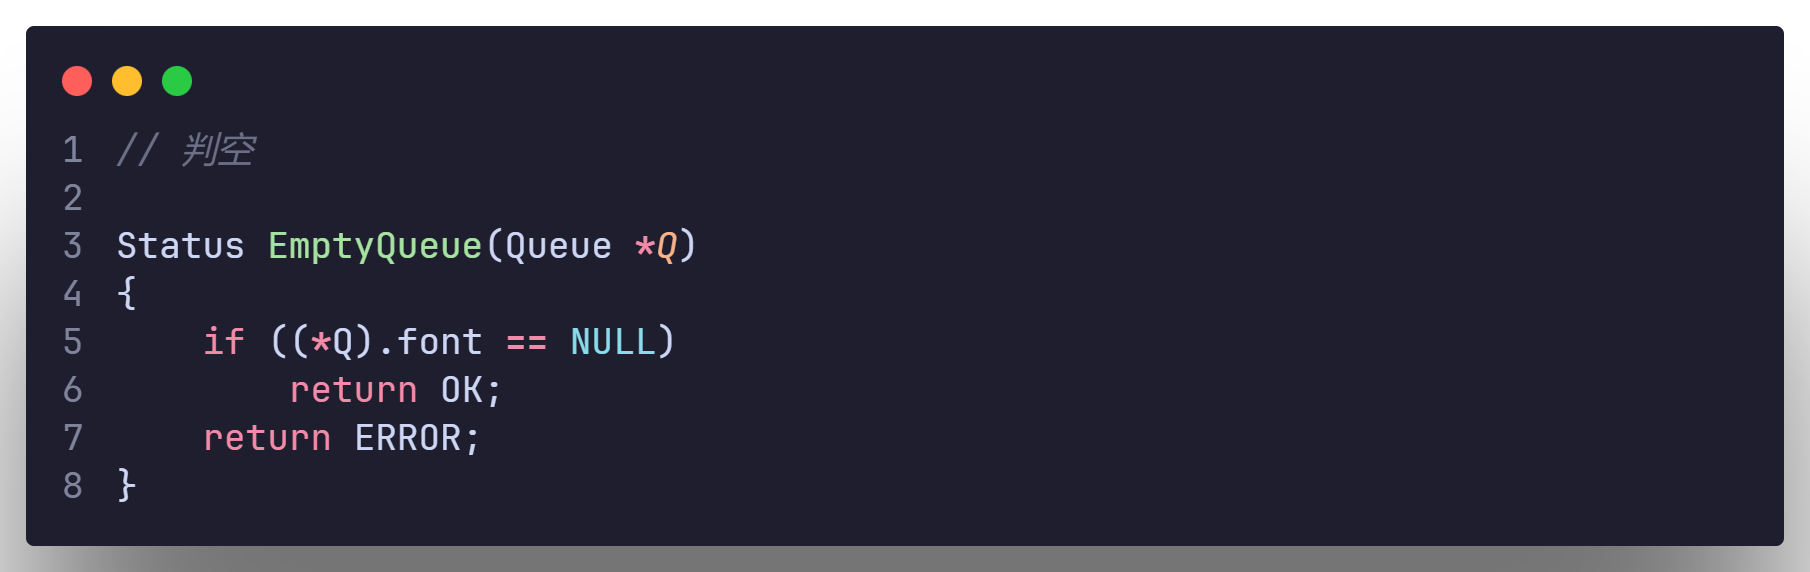
\includegraphics[scale=0.2]{"figure/Note/Stack/QlEmpty.png"}
\end{figure}

(4). 打印队列

\begin{figure}[H]
    \centering
    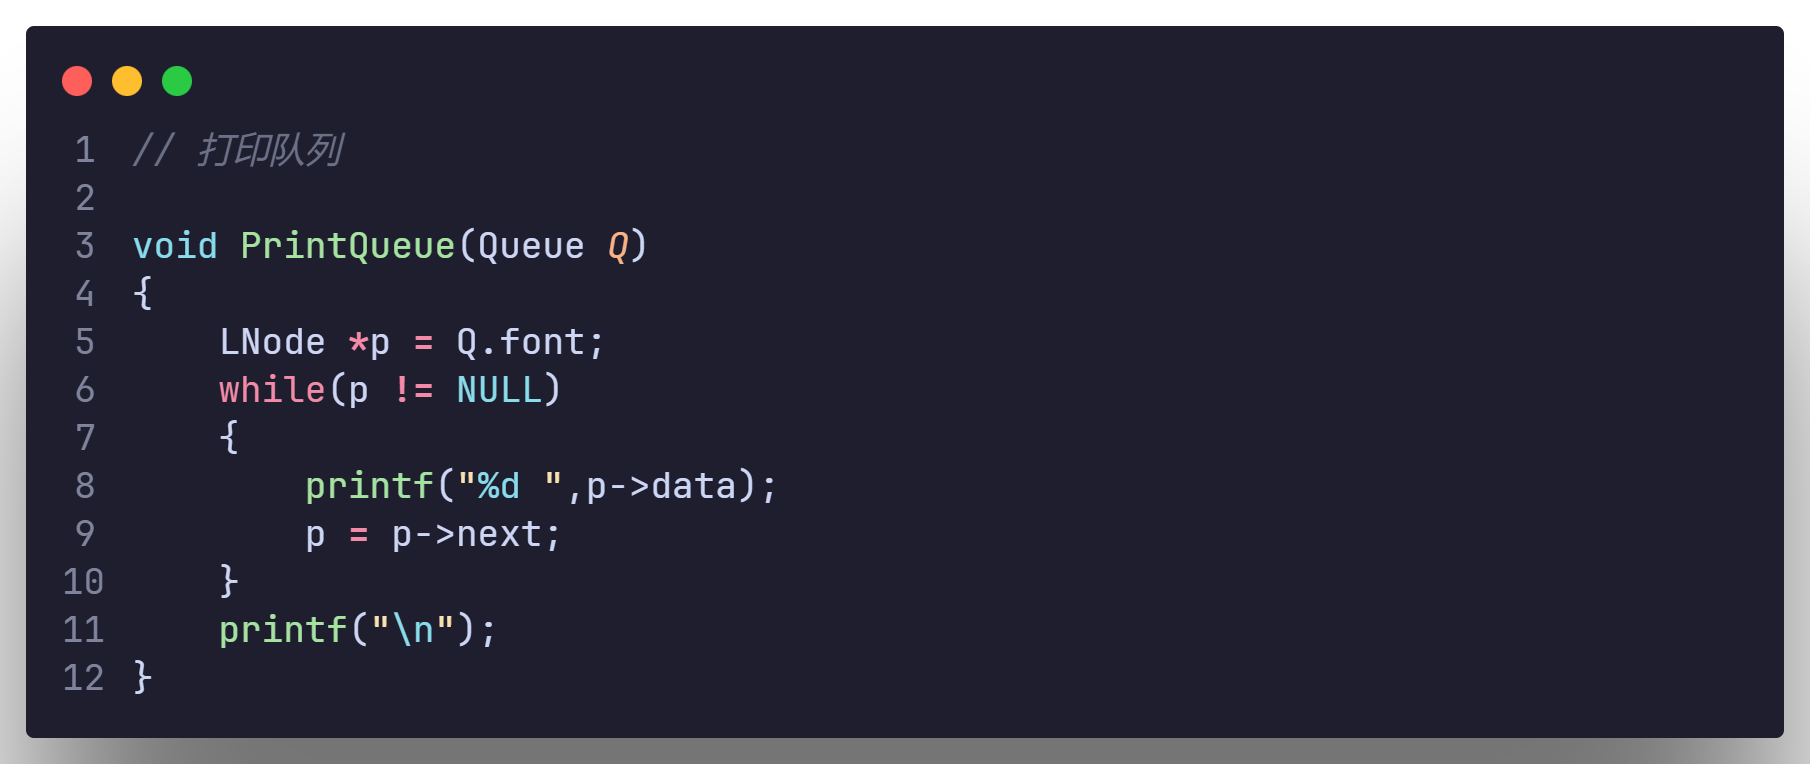
\includegraphics[scale=0.2]{"figure/Note/Stack/QlPrint.png"}
\end{figure}

\subsection{双端队列}
\begin{definition}[双端队列]
    双端队列是两端都能够插入和删除的队列, 一般采用链表或者顺序表实现, 只需要存储队头节点和队尾节点的指针

    \textbf{操作受限的双端队列:}
    \begin{enumerate}
        \item 只有一端可以插入, 两端可以删除的队列
        \item 只有一端可以删除, 两段可以插入的队列
    \end{enumerate}
\end{definition}
\section{栈和队列的应用}
\subsection{括号匹配}
\begin{theorem}[算法步骤]
    \begin{enumerate}
        \item 遇到左括号压栈, 遇到右括号出栈
        \item 如果出栈为空, 或者出栈元素和当前右括号不匹配, 返回错误
        \item 如果遍历完所有括号, 栈为空, 返回正确
    \end{enumerate}
\end{theorem}
\subsection{前缀、中缀、后缀表达式求值}
\begin{theorem}[表达式求值]
    一、前缀表达式: 运算符在前, 操作数在后
    \begin{enumerate}
        \item 从右向左扫描表达式, 遇到操作数入栈, 遇到运算符, 从栈中弹出两个操作数, 进行运算
        \item 第一个弹出的操作数是右操作数, 第二个弹出的操作数是左操作数, 运算结果入栈
        \item 最后栈中的元素就是表达式的值
    \end{enumerate}

    二、中缀表达式: 运算符在中间, 操作数在两边, 直接计算

    三、后缀表达式: 运算符在后, 操作数在前
    \begin{enumerate}
        \item 从左向右扫描表达式, 遇到操作数入栈, 遇到运算符, 从栈中弹出两个操作数, 进行运算
        \item 第一个弹出的操作数是左操作数, 第二个弹出的操作数是右操作数, 运算结果入栈
        \item 最后栈中的元素就是表达式的值
    \end{enumerate}
\end{theorem}

\subsection{表达式转换}
\begin{theorem}[表达式转换: 手算]
    一、中缀表达式 $\to$ 前缀表达式: 按照运算顺序, 从左向右扫描, 把操作符放在左边, 操作数放在右边, 将得到的前缀表达式作为操作数继续进行操作, 直到得到最终的前缀表达式

    二、中缀表达式 $\to$ 后缀表达式: 按照运算顺序, 从左向右扫描, 把操作符放在右边, 操作数放在左边, 将得到的后缀表达式作为操作数继续进行操作, 直到得到最终的后缀表达式

    三、前缀表达式 $\to$ 后缀表达式和 后缀表达式 $\to$ 前缀表达式: 先将前缀表达式转换为中缀表达式, 再将中缀表达式转换为后缀表达式; 同理可以将后缀表达式转换为前缀表达式

\end{theorem}
\subsection{队列应用}
\begin{definition}[队列应用]
    1. 树的层次遍历, 按照根节点入队,出队,再将左右孩子入队,出队,直到队列为空

    2. 图的广度优先搜索, 按照顶点入队,出队,再将与该顶点相邻的顶点入队,出队,直到队列为空

    3. 模拟操作系统的进程调度, 先到的进程先执行,后到的进程后执行($\mathbf{FCFS}$)

    4. 图的深度有限搜索, 按照顶点入栈,出栈,再将与该顶点相邻的顶点入栈,出栈,直到栈为空
\end{definition}

\section{数组}
\begin{definition}[数组]
    数组是由类型相同的元素构成的有序集合, 每个元素称为数组元素, 每个元素有唯一下标, 可通过下标访问该数据元素; 
    一维数组可以看作线性表; 二维数组是数据元素为一维数组的线性表
\end{definition}
$$LOC(i,j) = LOC(0,0) + (n\times i + j)L$$

\subsection{特殊矩阵的压缩}
\subsubsection{对称矩阵}

$a_{ij}$ 在数组中的下标 $k$

$$ k =
\begin{cases}
    \dfrac{i(i-1)}{2}+j-1, & i\geq j\\
    \dfrac{j(j-1)}{2}+i-1, & i<j\ (a_{ij}=a_{ji})
\end{cases}
$$

\subsubsection{三角矩阵}

(1). 上三角矩阵

$a_{ij}$在数组中的下标$k$:

$$ k = 
\begin{cases}
    \dfrac{(i-1)(2n-i+2)}{2}+j-i, & i\leq j\\
    \dfrac{n(n+1)}{2},            & i > j\ (a_{ij}=c)
\end{cases}
$$

(2). 下三角矩阵

$a_{ij}$在数组中的下标$k$:

$$ k = 
\begin{cases}
    \dfrac{i(i-1)}{2}+j-1, & i\geq j\\
    \dfrac{n(n+1)}{2},     & i < j\ (a_{ij}=c)
\end{cases}
$$

\subsubsection{对称矩阵}

(1). 三对角矩阵

$a_{ij}$ 在数组中的下标 $k$:

$$ k = 
\begin{cases}
    2i+j-3, & |i-j| \leq 1\\
    3n-2,   & |i-j| > 1
\end{cases}
$$

已知数组下标 $k$ 时:

$$\begin{cases}
    i = [\dfrac{k+1}{3}]+1\\
    j = k-2i+3
\end{cases}$$

\subsubsection{稀疏矩阵}

采用三元组的方式存储, 不仅需要存储数据, 还需要存储行号和列号以及非零元素的个数, 失去随机存储的特性
\begin{table}[ht]
    \centering
    \begin{tabular}{>{\centering\arraybackslash}p{1cm} >{\centering\arraybackslash}p{1cm} >{\centering\arraybackslash}p{2cm}}
    \toprule
    \rowcolor[HTML]{FCE5CD} 
    \textit{i} & \textit{j} & \textit{num} \\ 
    \midrule
    \rowcolor[HTML]{FFF2CC} 
    0 & 0 & 4 \\ 
    \rowcolor[HTML]{FCE5CD} 
    1 & 2 & 6 \\ 
    \rowcolor[HTML]{FFF2CC} 
    2 & 1 & 9 \\ 
    \rowcolor[HTML]{FCE5CD} 
    3 & 1 & 23 \\ 
    \bottomrule
    \end{tabular}
\end{table}

\section{栈和队列可视化}
\begin{enumerate}
    \item \href{https://www.cs.usfca.edu/~galles/visualization/StackArray.html}{数组栈}
    \item \href{https://www.cs.usfca.edu/~galles/visualization/StackLL.html}{链表栈}
    \item \href{https://www.cs.usfca.edu/~galles/visualization/QueueArray.html}{数组队列}
    \item \href{https://www.cs.usfca.edu/~galles/visualization/QueueLL.html}{链表队列}
\end{enumerate}